\section{Implementation}

The following section outlines the key steps for capturing
depth images, converting them into point clouds and using these point clouds
for 3D reconstruction.

\subsection{Depth Images}
 The workings of the previous generation of RealSense cameras are detailed in \cite{keselman2017intel}.
The algorithm described therein has not significantly changed (I believe) in the 400 series.
The new features seem to be additional on-device hardware post-processing.

These cameras produce four-channel image composed of the standard RGB colour channels together with a fourth depth channel. The depth channel associates to each pixel an estimate of the distance from the camera to the surface.

The D435 (and similar available devices) use a stereoscopic technique inspired by human
binocular vision.
It is possible to compute a pixel's depth by comparing the images produced by two cameras placed at known distances and pointing in generally the same direction. After projecting the images onto a common plane (the cameras produce images which are slightly ``angled''), the camera computes the \textit{disparity}
 $d$ between the two images.

\begin{figure}[h]
 \centering
 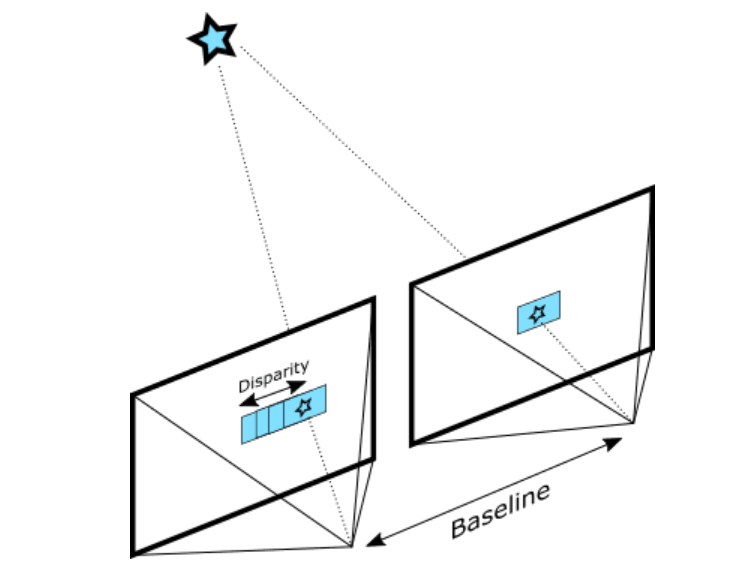
\includegraphics[width=0.45\textwidth]{binocular_vision.png}
 \caption{Binocular Vision}
 \end{figure}

Disparity is the distance (in pixels) of a cluster of pixels from one image to the other.
Objects closer to the camera will have greater disparity between the two images, distant
objects less so.
With distance $B$ between the two cameras and the focal length $f$, the disparity allows the camera
to infer the depth $z$ using the formula:

\[ z = \frac{f \cdot B}{d} \]

However, this simple stereoscopic approach struggles in many different
environments. When materials are transparent, reflective or patterned, or occluded,
the algorithm can struggle to find meaningful clusters of disparity.
To improve the robustness of the depth calculation on a variety
of textures and surfaces, the devices additionally include an infrared projector.

\begin{figure}[h]
\centering
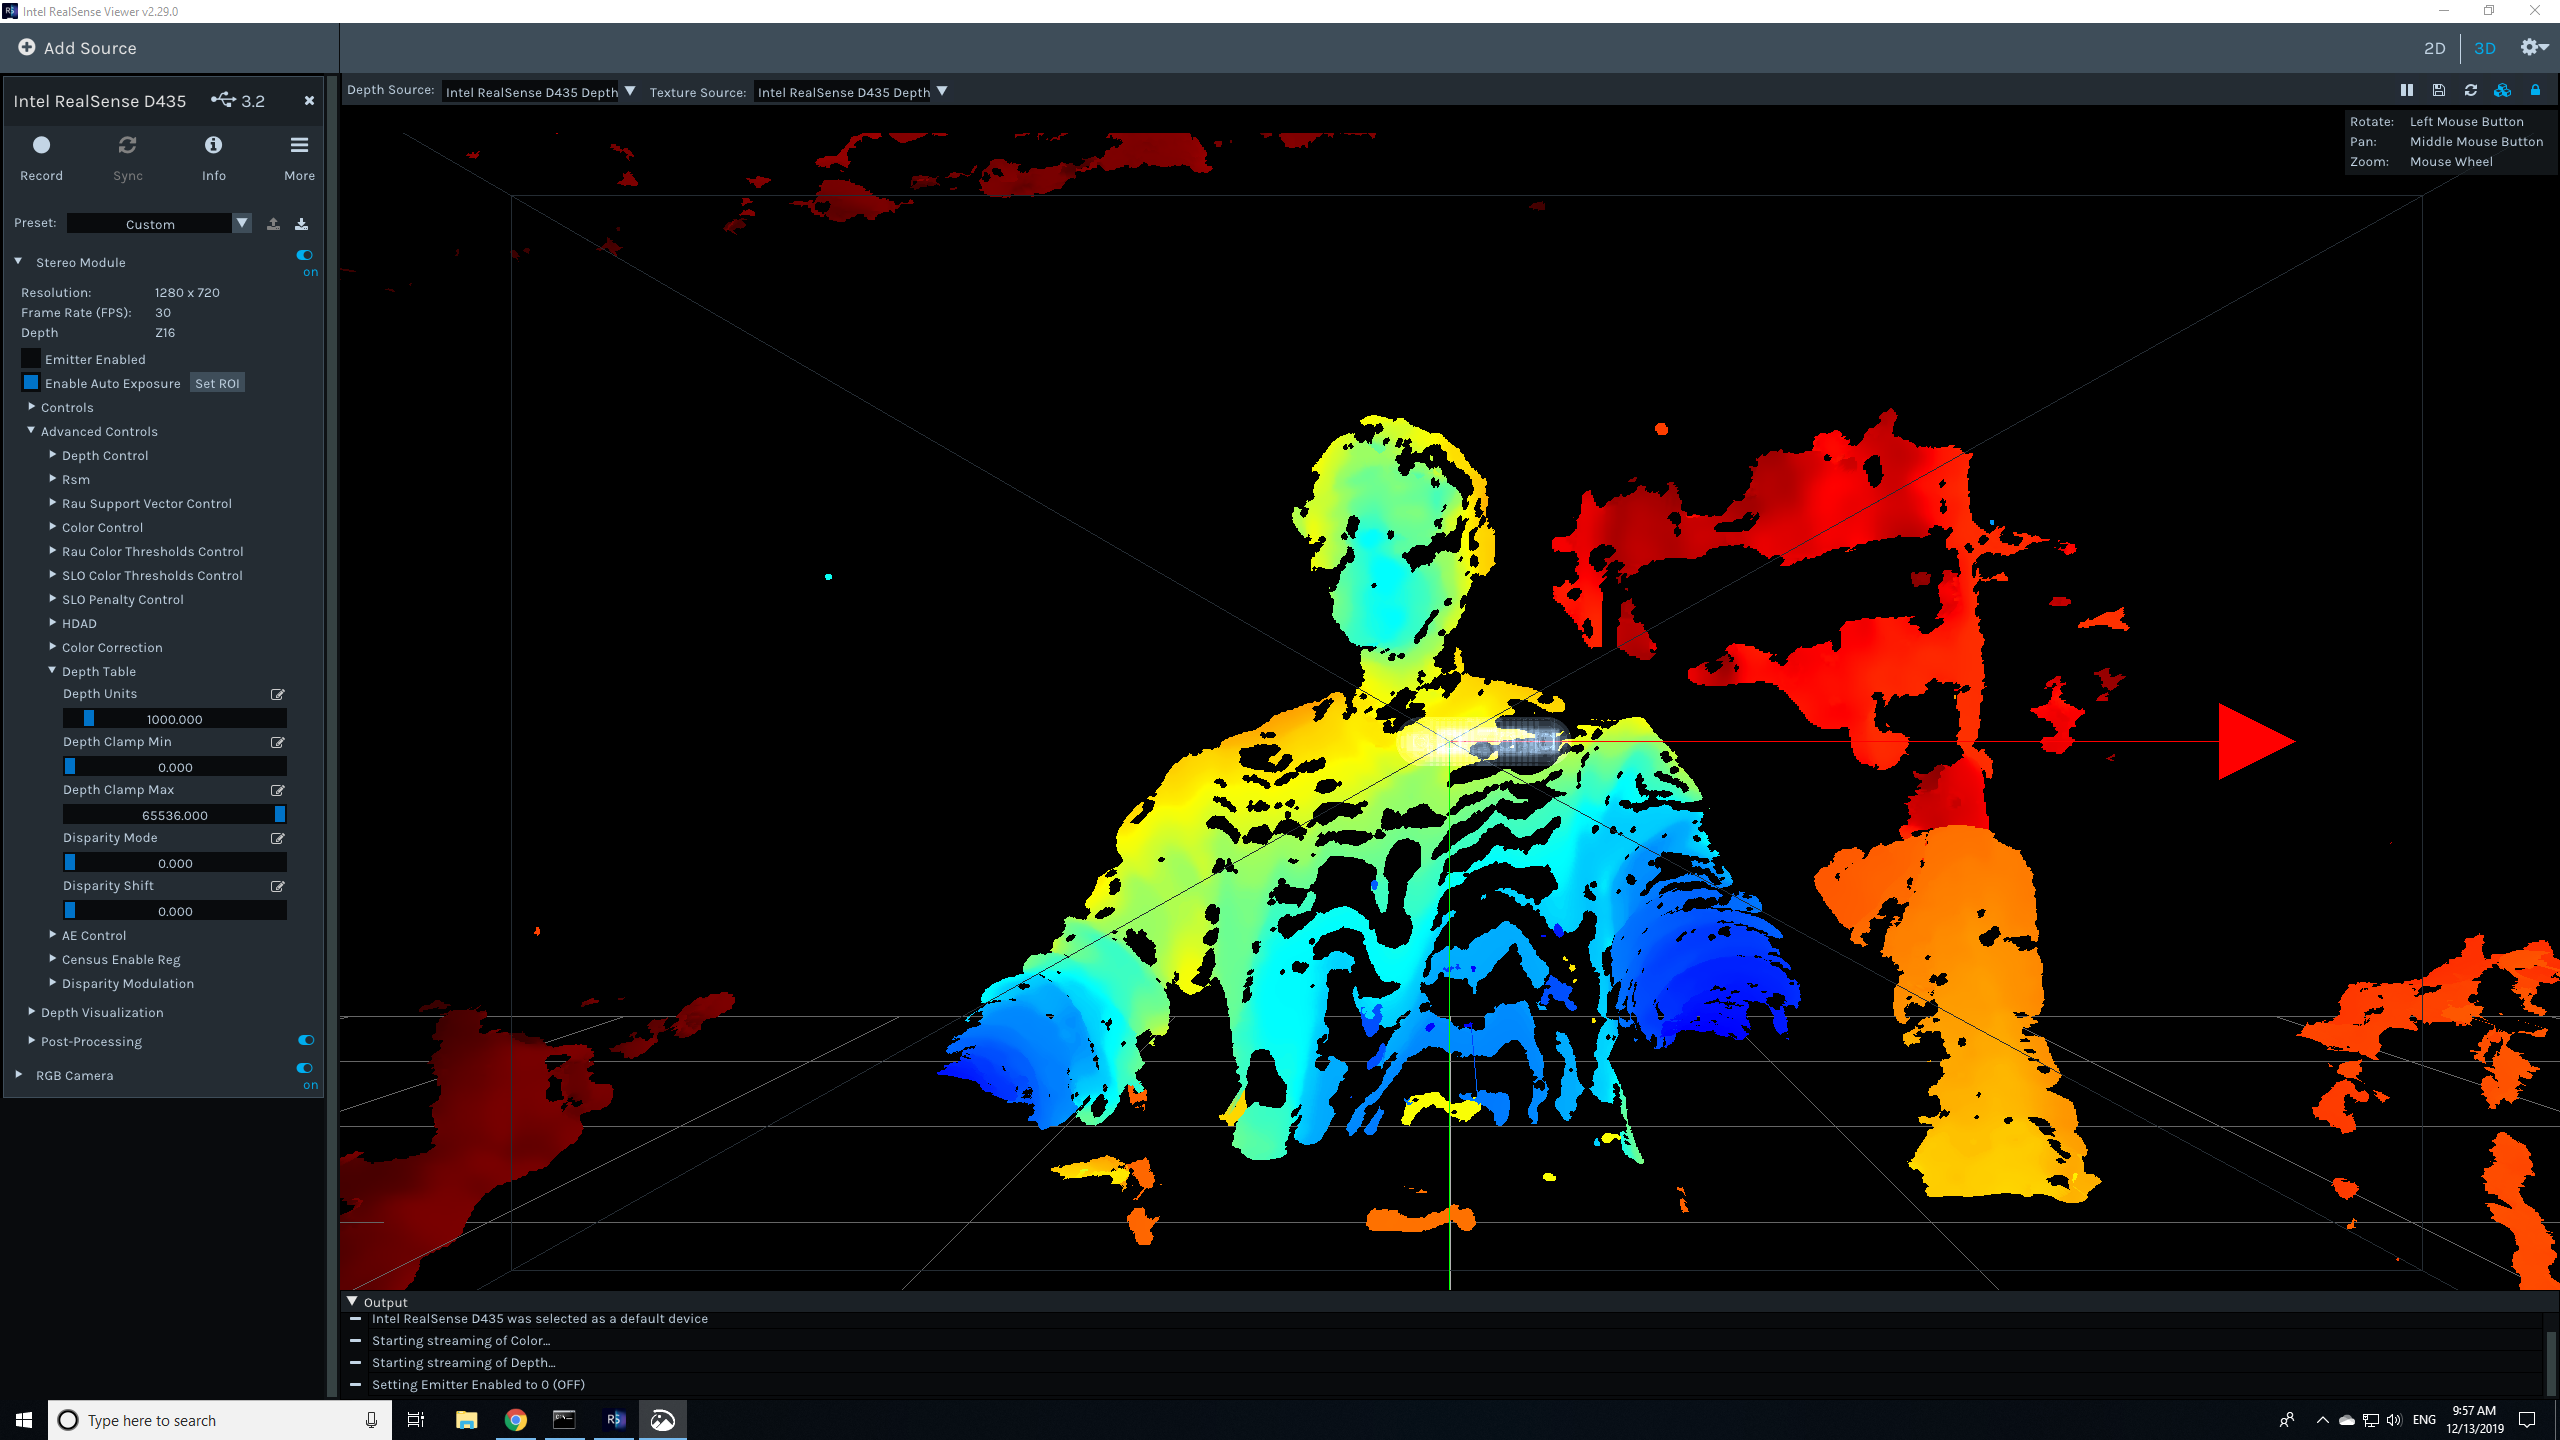
\includegraphics[width=0.35\textwidth]{without_emitter.png}
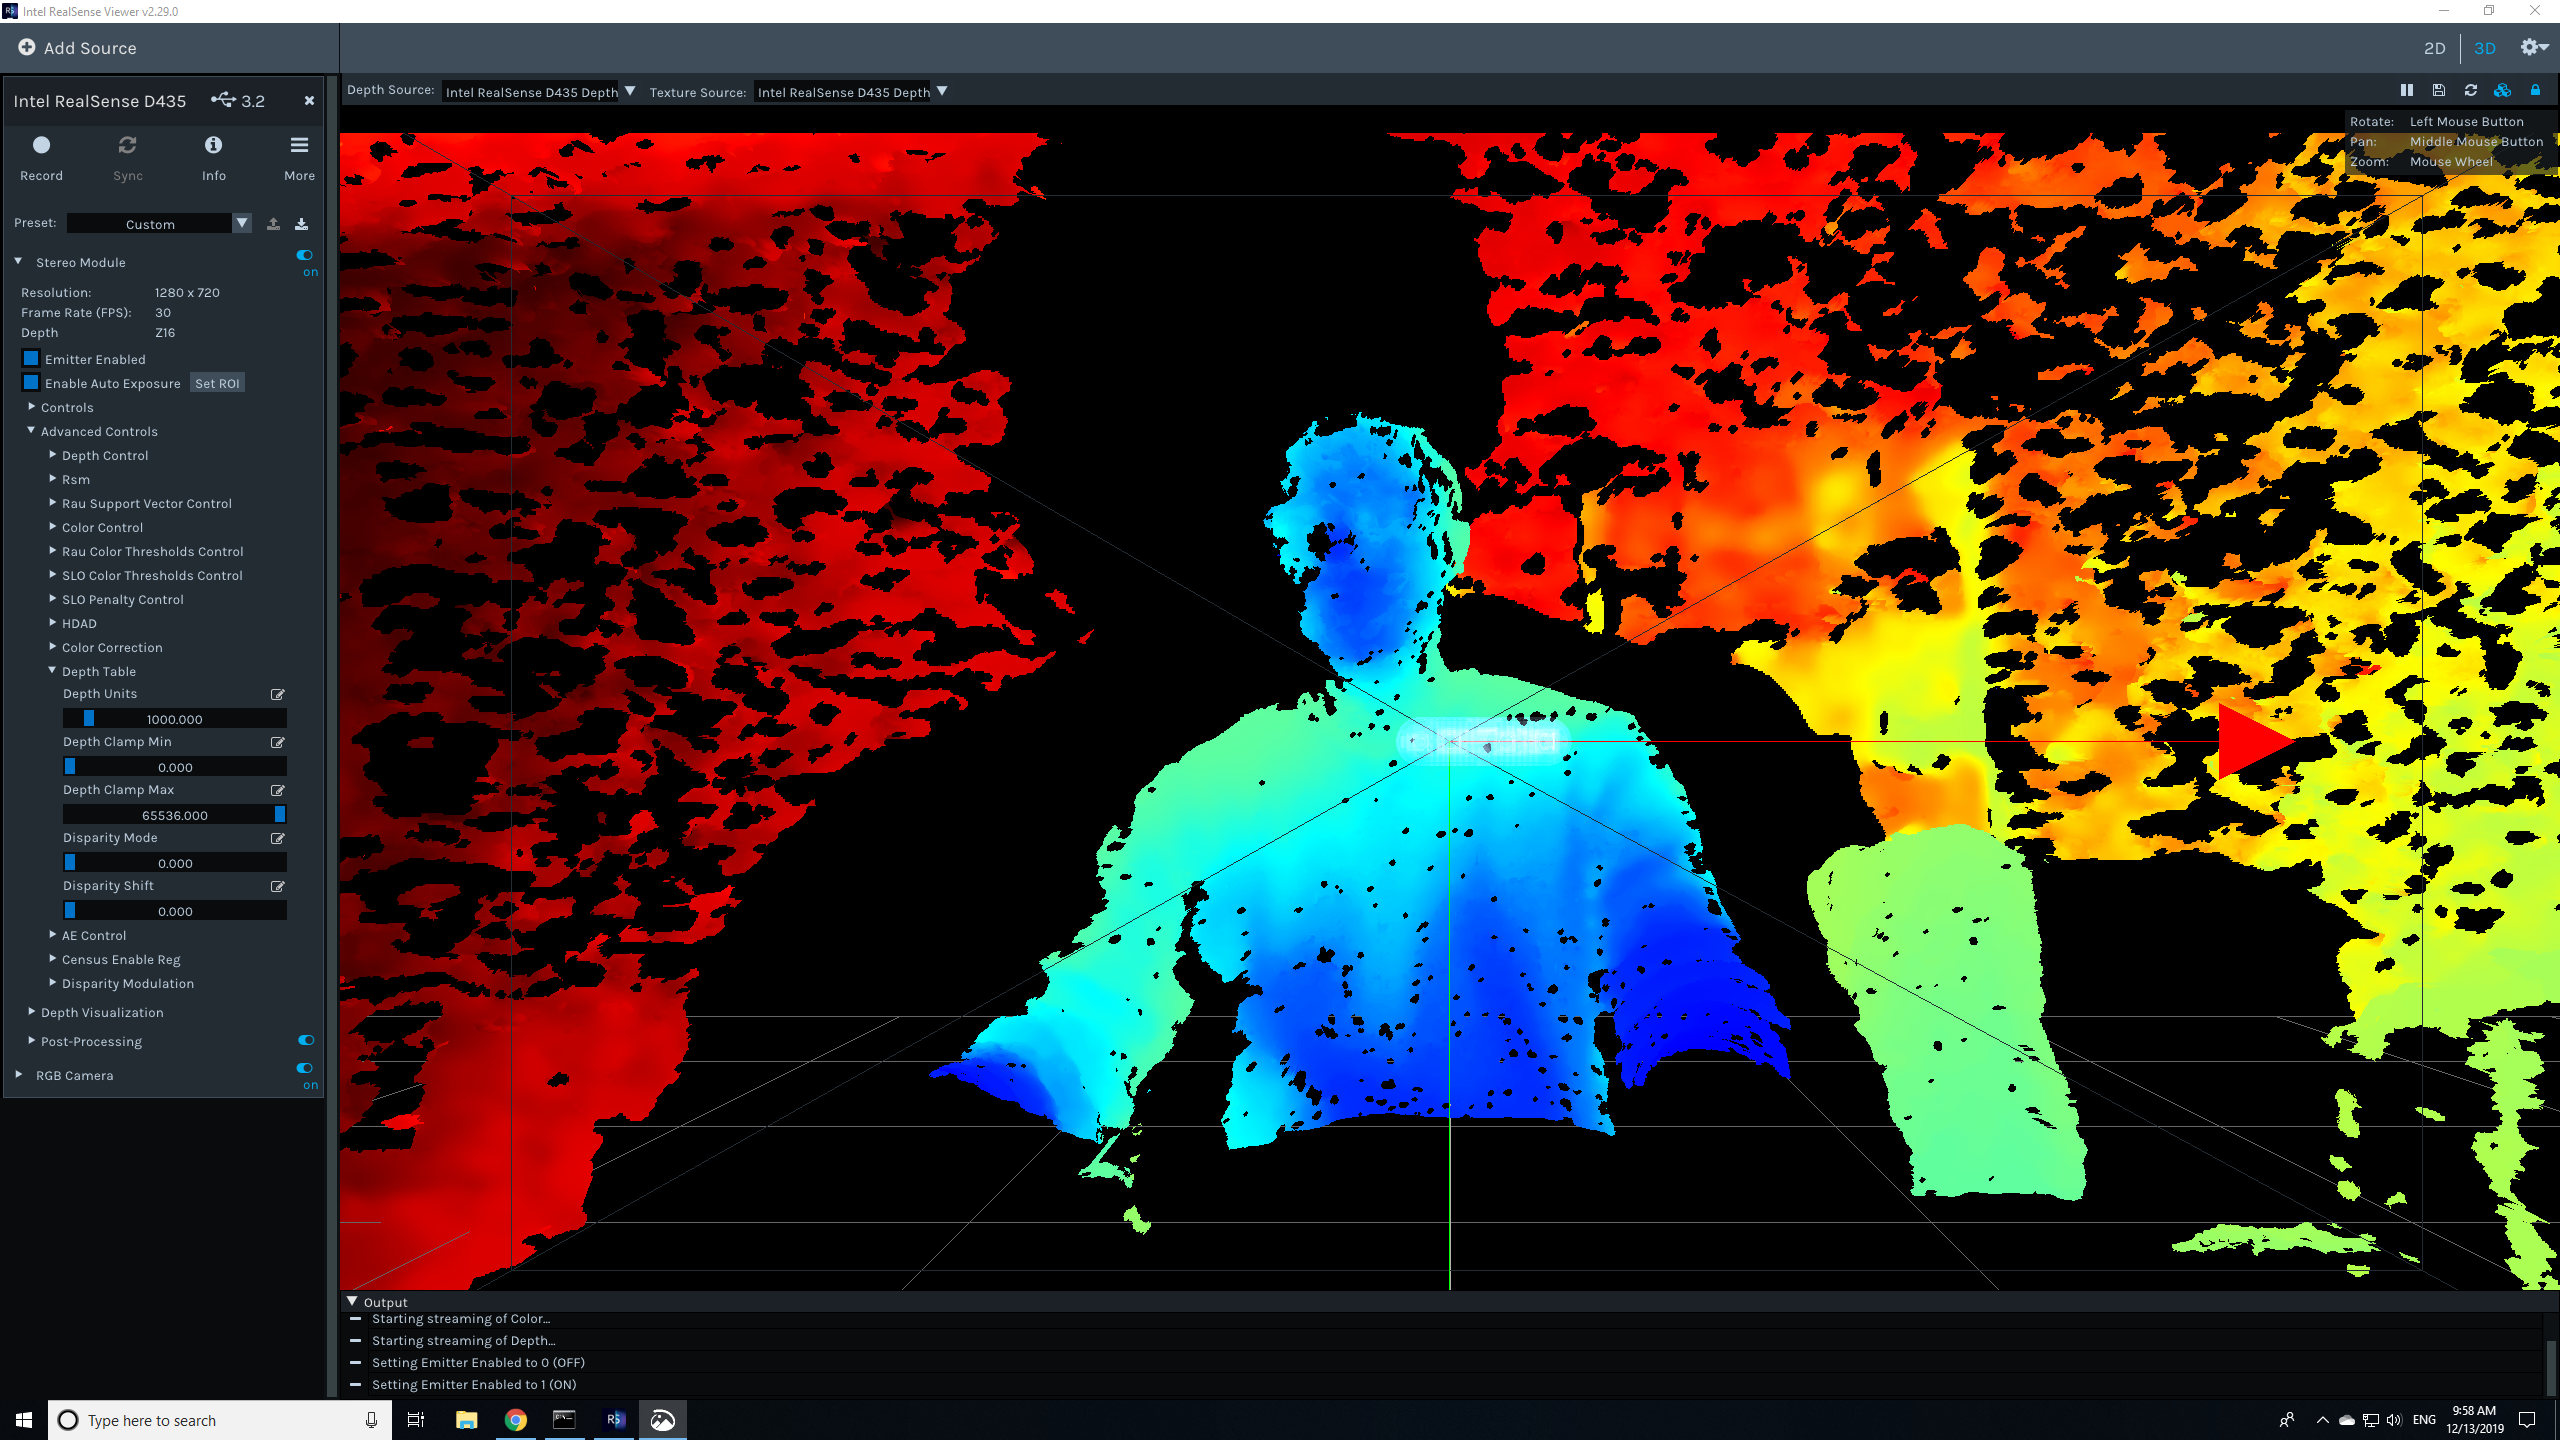
\includegraphics[width=0.35\textwidth]{with_emitter.png}
\caption{Infrared emitter on (left) and off (right)}
\end{figure}

In the pictures above, you can see that without the emitter, the camera is
unable to detect the uniformly white wall behind me. The emitter allows the camera
to make measurements, but notice how the unstructured infrared light adds a rippling
distortion to the measurements.

All of the complexity of these calculations, of course, are abstracted in the Viewer
and SDK bundled with the camera.
Using the Intel software, it is straightforward to take depth-snapshots or videos
and export them to mesh files.

\subsection{Depth Pixel to Point Cloud Transformation}
With the $x$ and $y$ coordinates of a pixel and a corresponding depth measurement $z$,
it is possible to apply a transformation to obtain a point in a 3d frame of
reference, say, ``in front of the camera''.

This transformation depends on the configuration and specifications of the camera(s).
Suffice it to say that the RealSense SDK and Viewer offer functions which can
convert from 2d pixel space to 3d space.

Note that this conversion may involve a tradeoff. Each pixel's frustum is a thin but expanding shape so closer pixels are smaller than distant ones. Sophisticated transformations take this into consideration when converting depth values into voxels or points.

It may be of interest that the RealSense SDK offers a CUDA implementation at:

\url{github.com/IntelRealSense/librealsense/blob/master/src/cuda/cuda-pointcloud.cu}

This version runs the per-pixel conversion on the GPU. The \textit{device} function
\begin{lstlisting}
deproject_pixel_to_point_cuda(float points[3], rs2_intrinsics,
  float pixel[2], float depth)
\end{lstlisting}
performs the per-point computation and the \textit{global} function
\begin{lstlisting}
kernel_deproject_depth_cuda(float * points, rs2_intrinsics*,
  uint16_t * depth, float depth_scale)
\end{lstlisting}
can be used to run a calculation on the GPU after allocating memory on the graphics device and
defining the number of cores/thread blocks to use. Both share an \textit{intrisic} object which stores the specifications of the camera and current frame.

\subsection{Background subtraction}

In order to align the different point clouds, it is necessary to remove noise and
outliers. We do not want error points to be considered when attempting align clouds.
When scanning an object in a room, the background, floor, and other features
of the room are noise.

Background subtraction is a well-studied problem in image computation \cite{piccardi2004background}.
A more sophisticated approach would adopt some of those techniques, such as
first taking an ``empty'' snapshot and subtracting it from subsequent ones to
isolate the model. More complicated approaches construct models of the background
to accomodate for change over time and so on.

\begin{figure}[h]
\centering
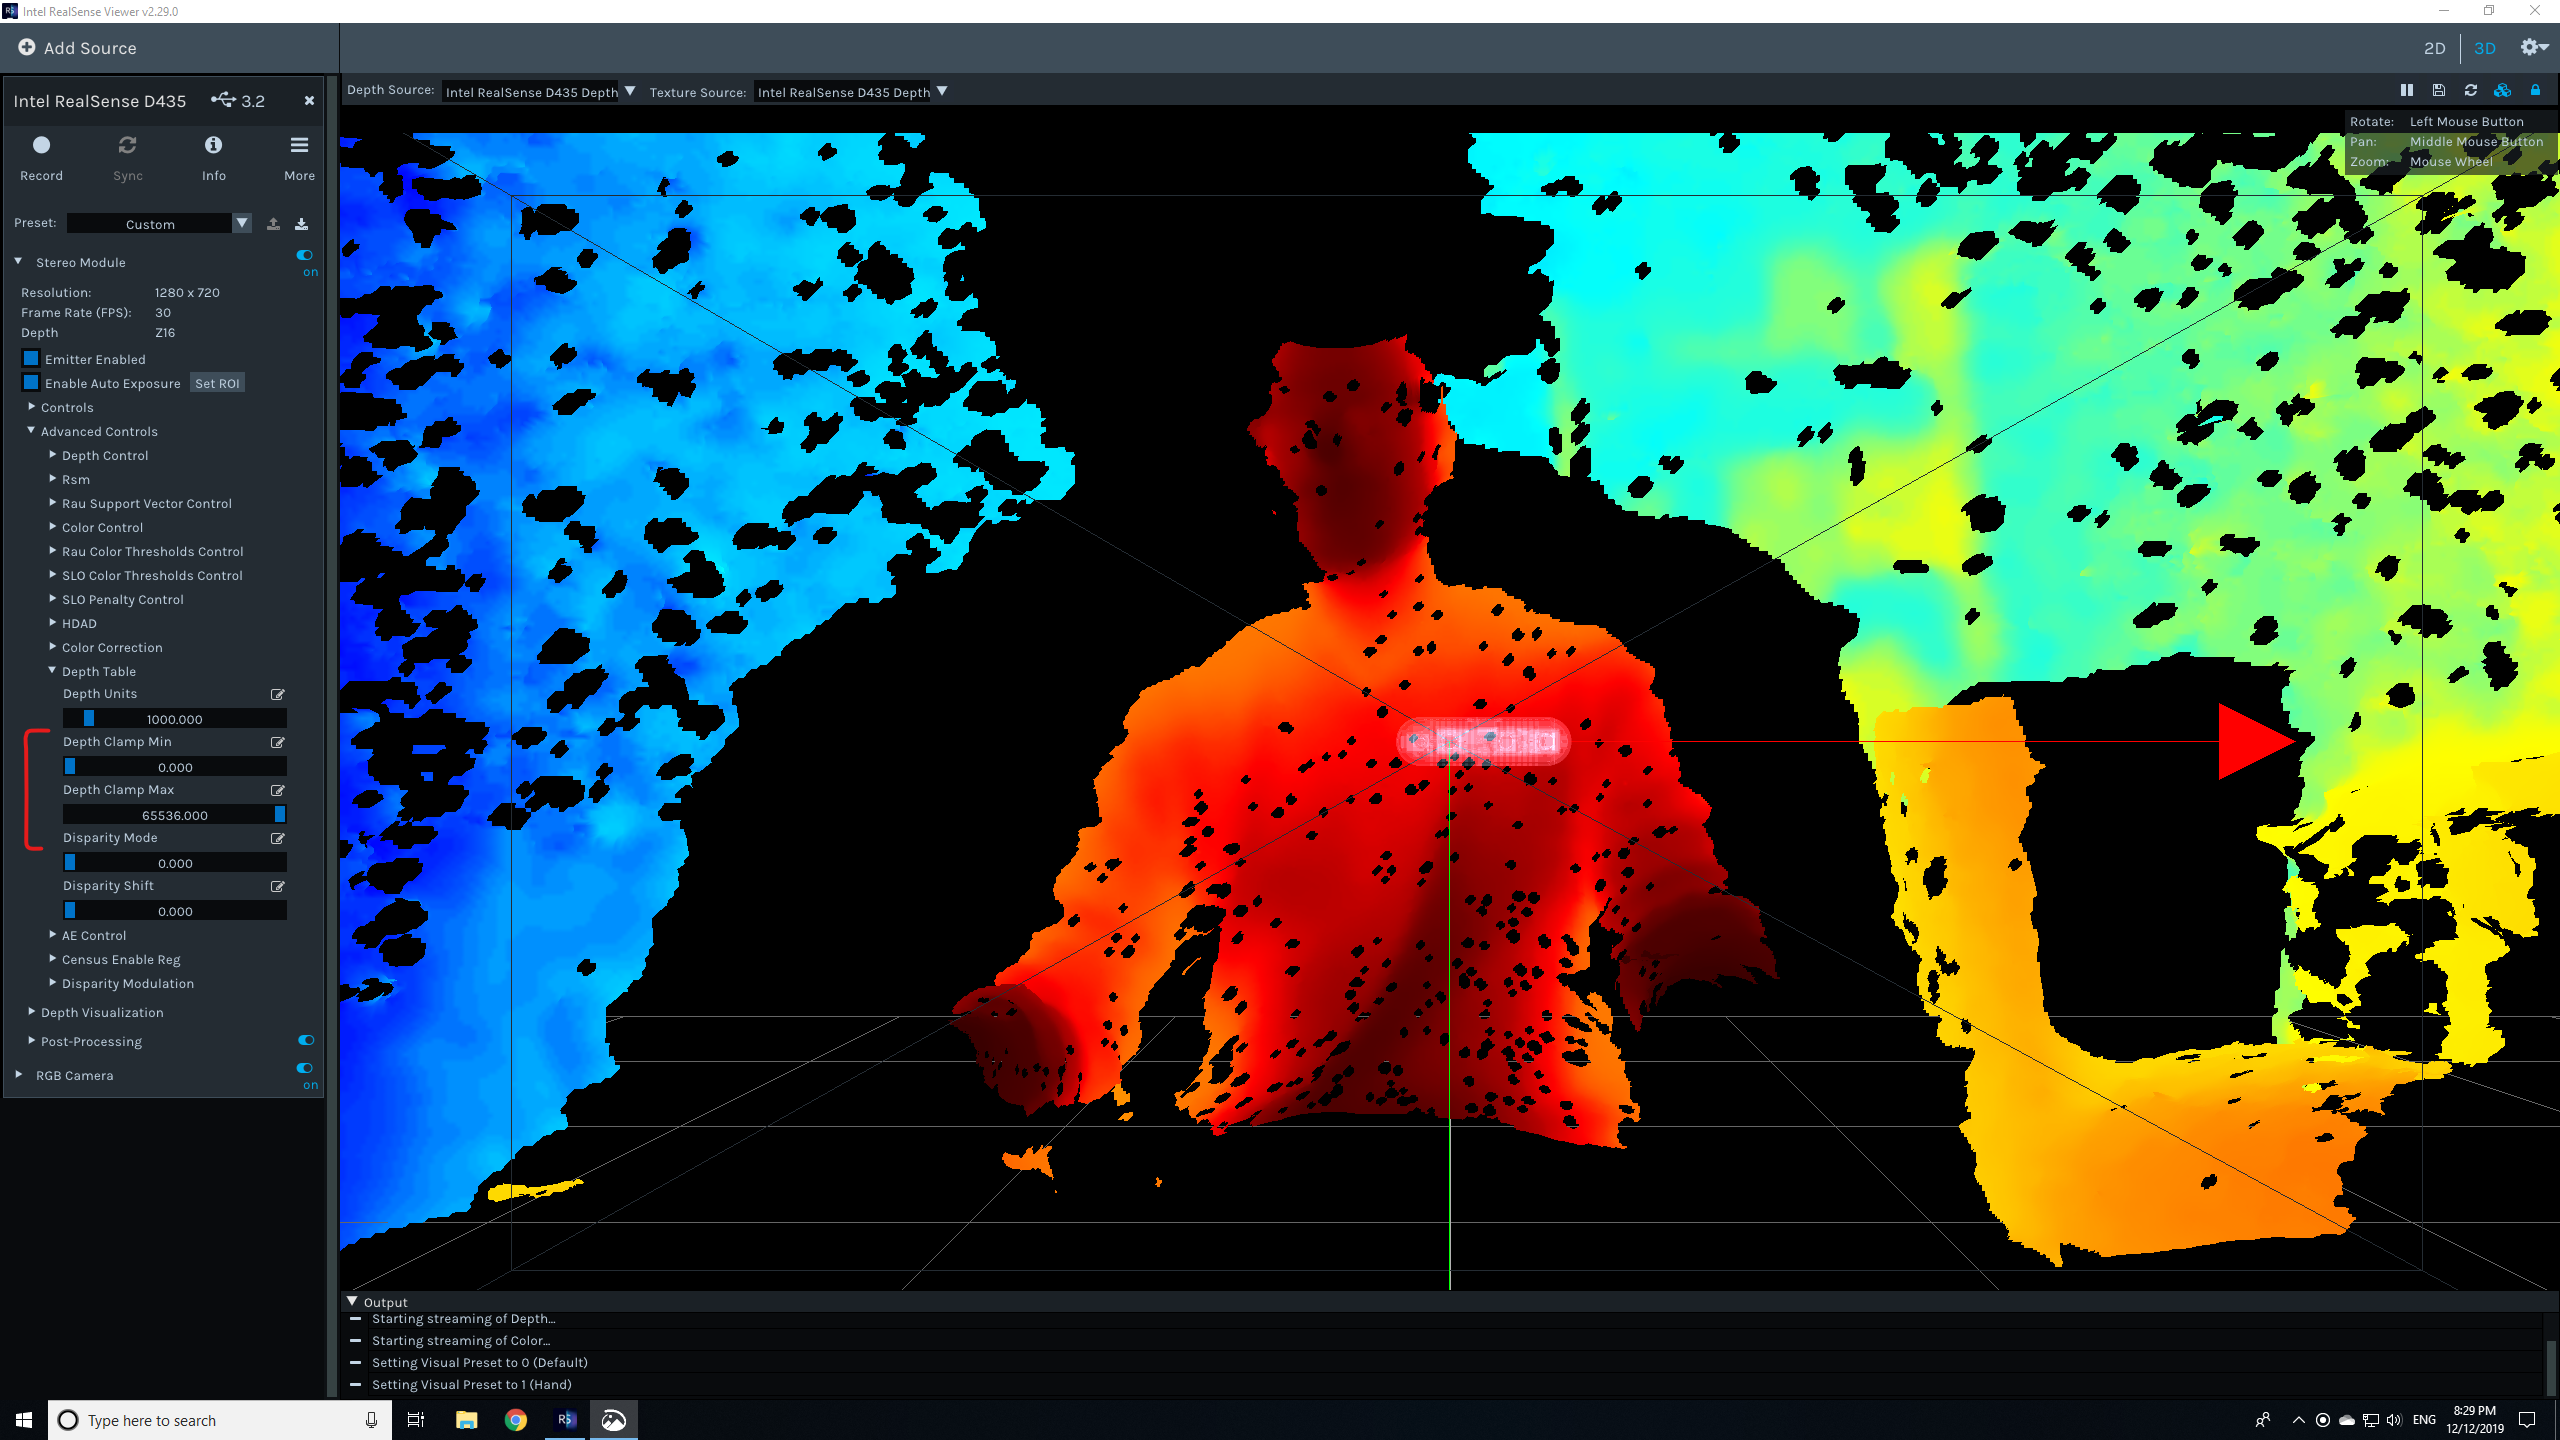
\includegraphics[width=0.45\textwidth]{max_depth_1.png}
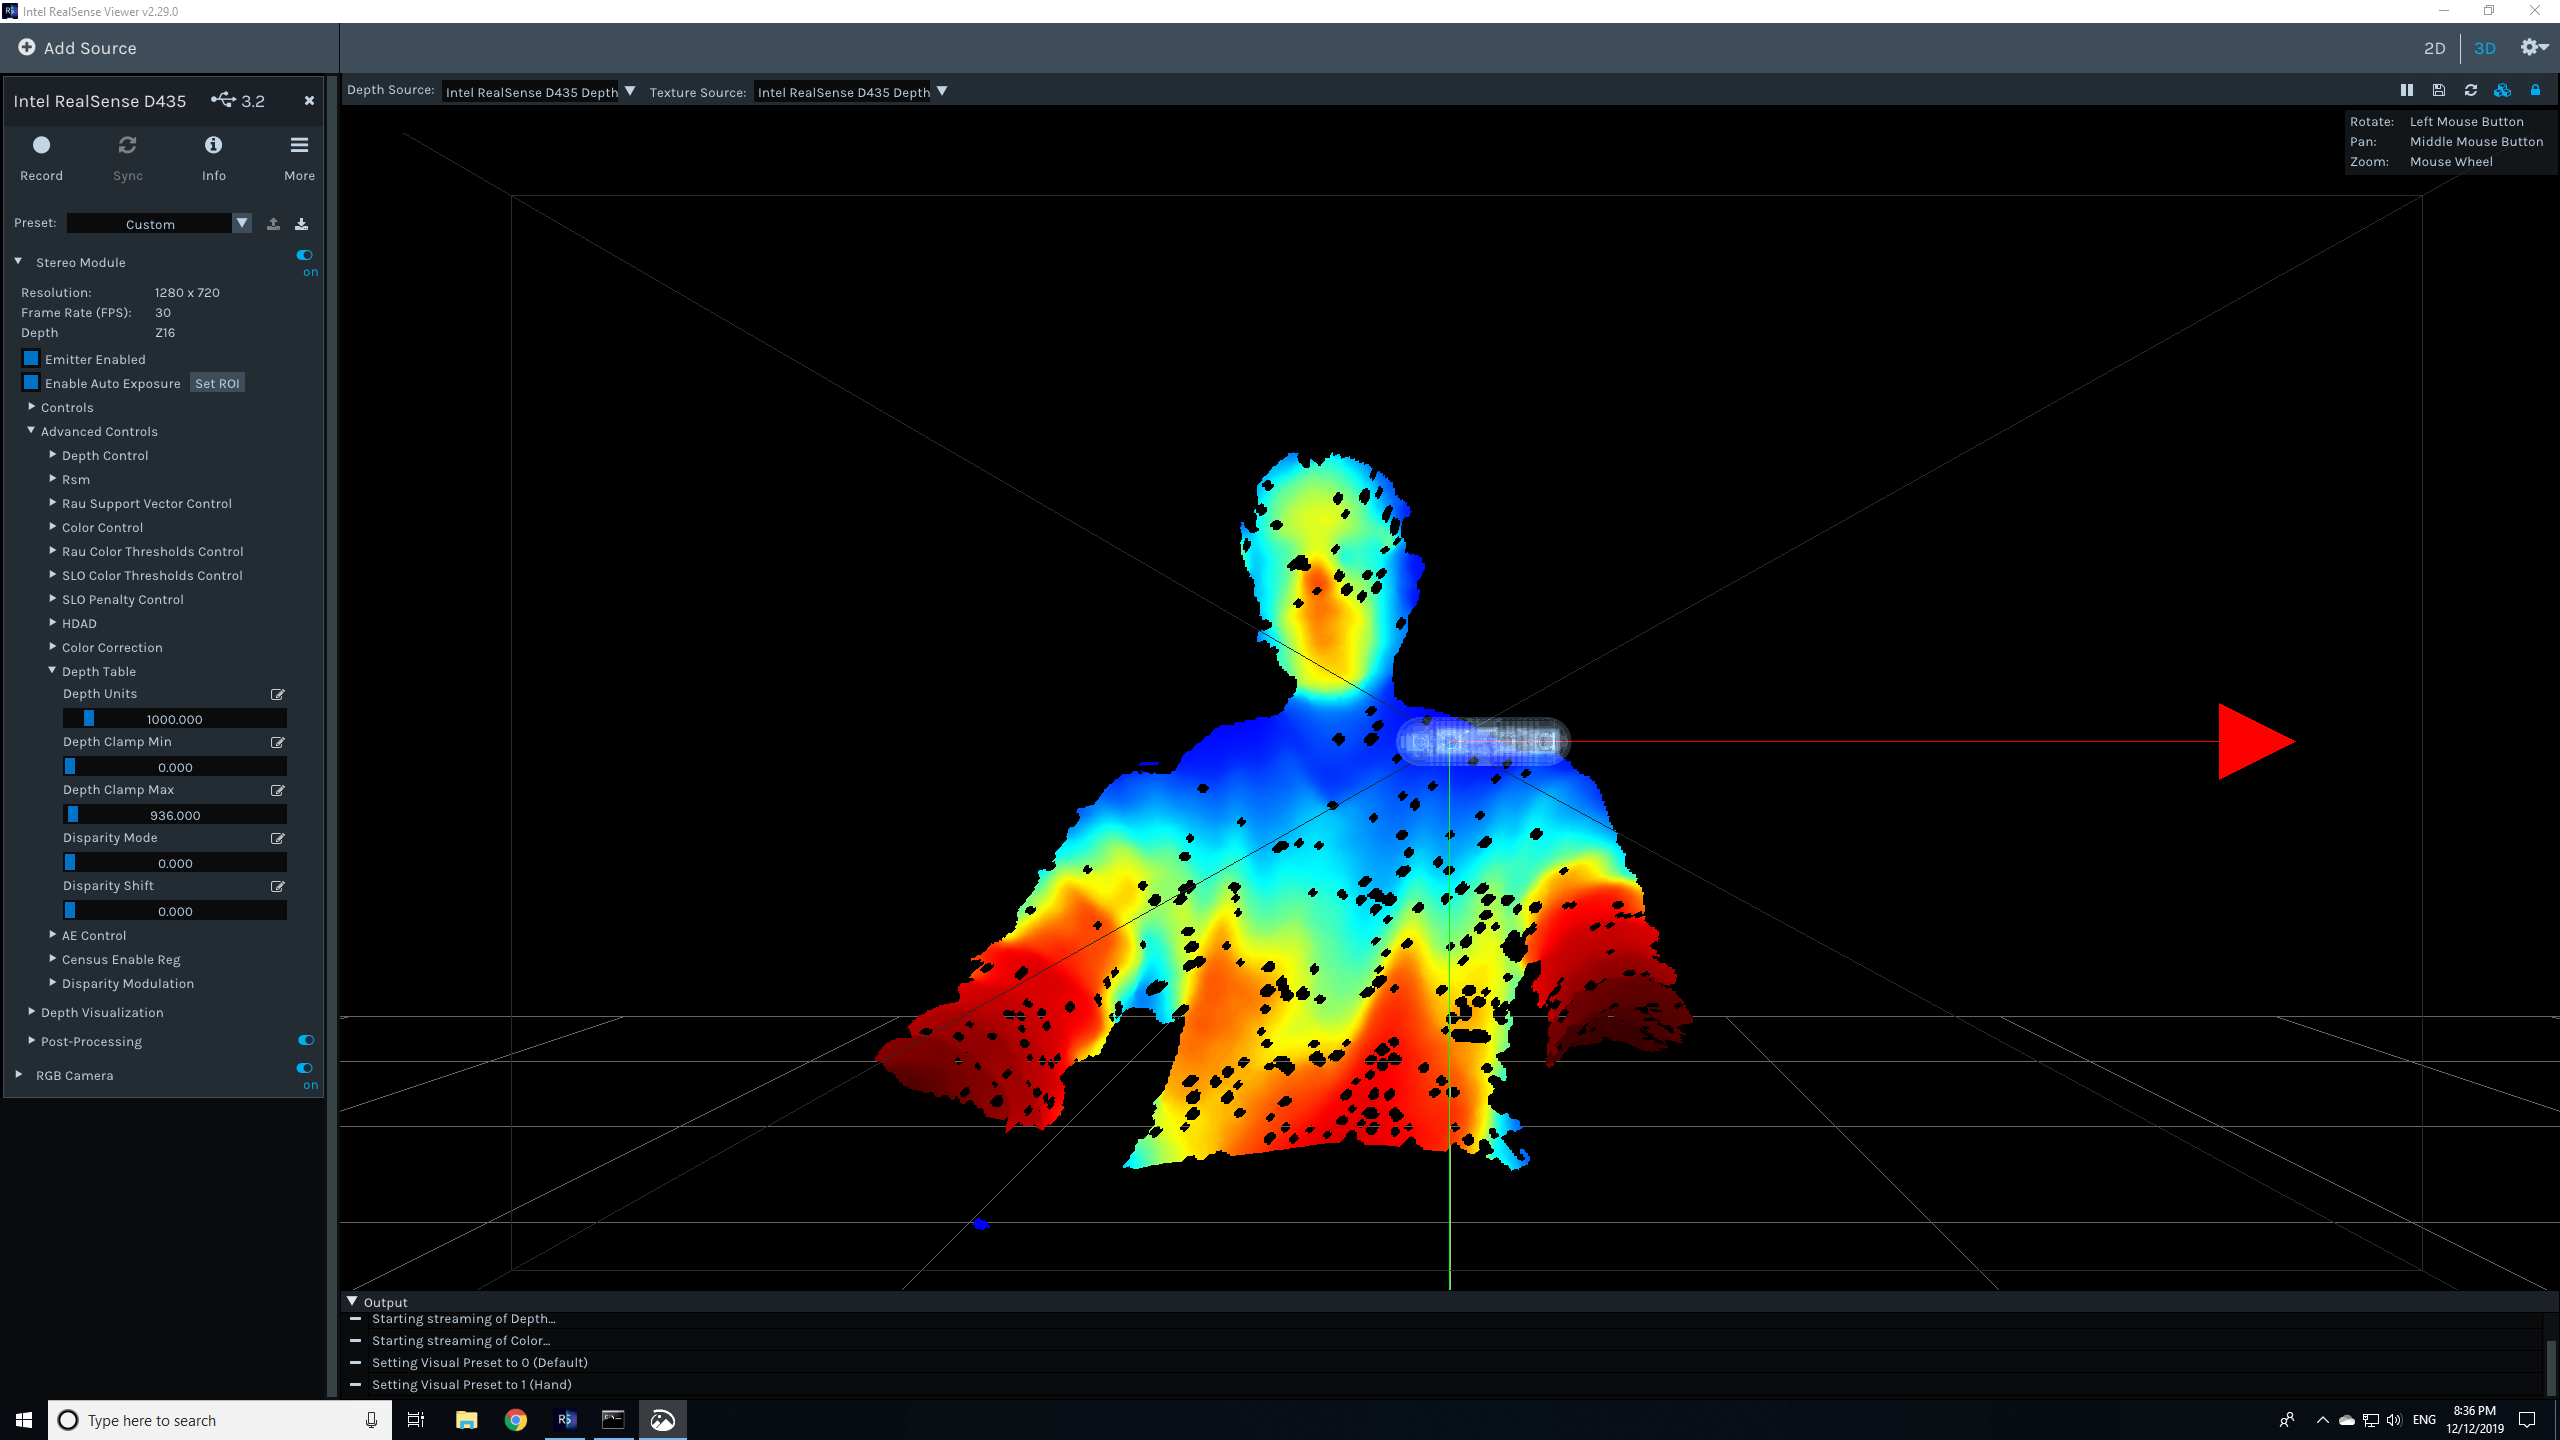
\includegraphics[width=0.45\textwidth]{max_depth_2.png}
\caption{Culling the back wall with max depth clamp}
\end{figure}

For our purpose of capturing toy examples, it suffices to set a maximum depth
and discard the back wall of a fixed scene. The RealSense Viewer allows the user
to pause a 3d scene and export a point cloud to ``.ply'' format. It's also possible to do this programmatically using the SDK: a modified version of the librealsense \text{pointcloud} example
takes a number of delayed snapshots (included below in Appendix).

\subsection{Filters}

The SDK and Viewer offer several post-processing filters to improve the quality of
the captured depth data. The spatial filter compares each pixel to its neighbours in a
frame to ensure that there are no improbable measurements. Temporal filters
compare new frames to some average or distribution of previous ones. The temporal
filter in particular reduces the flickering and warping of depth streams.

\begin{figure}[h]
\centering
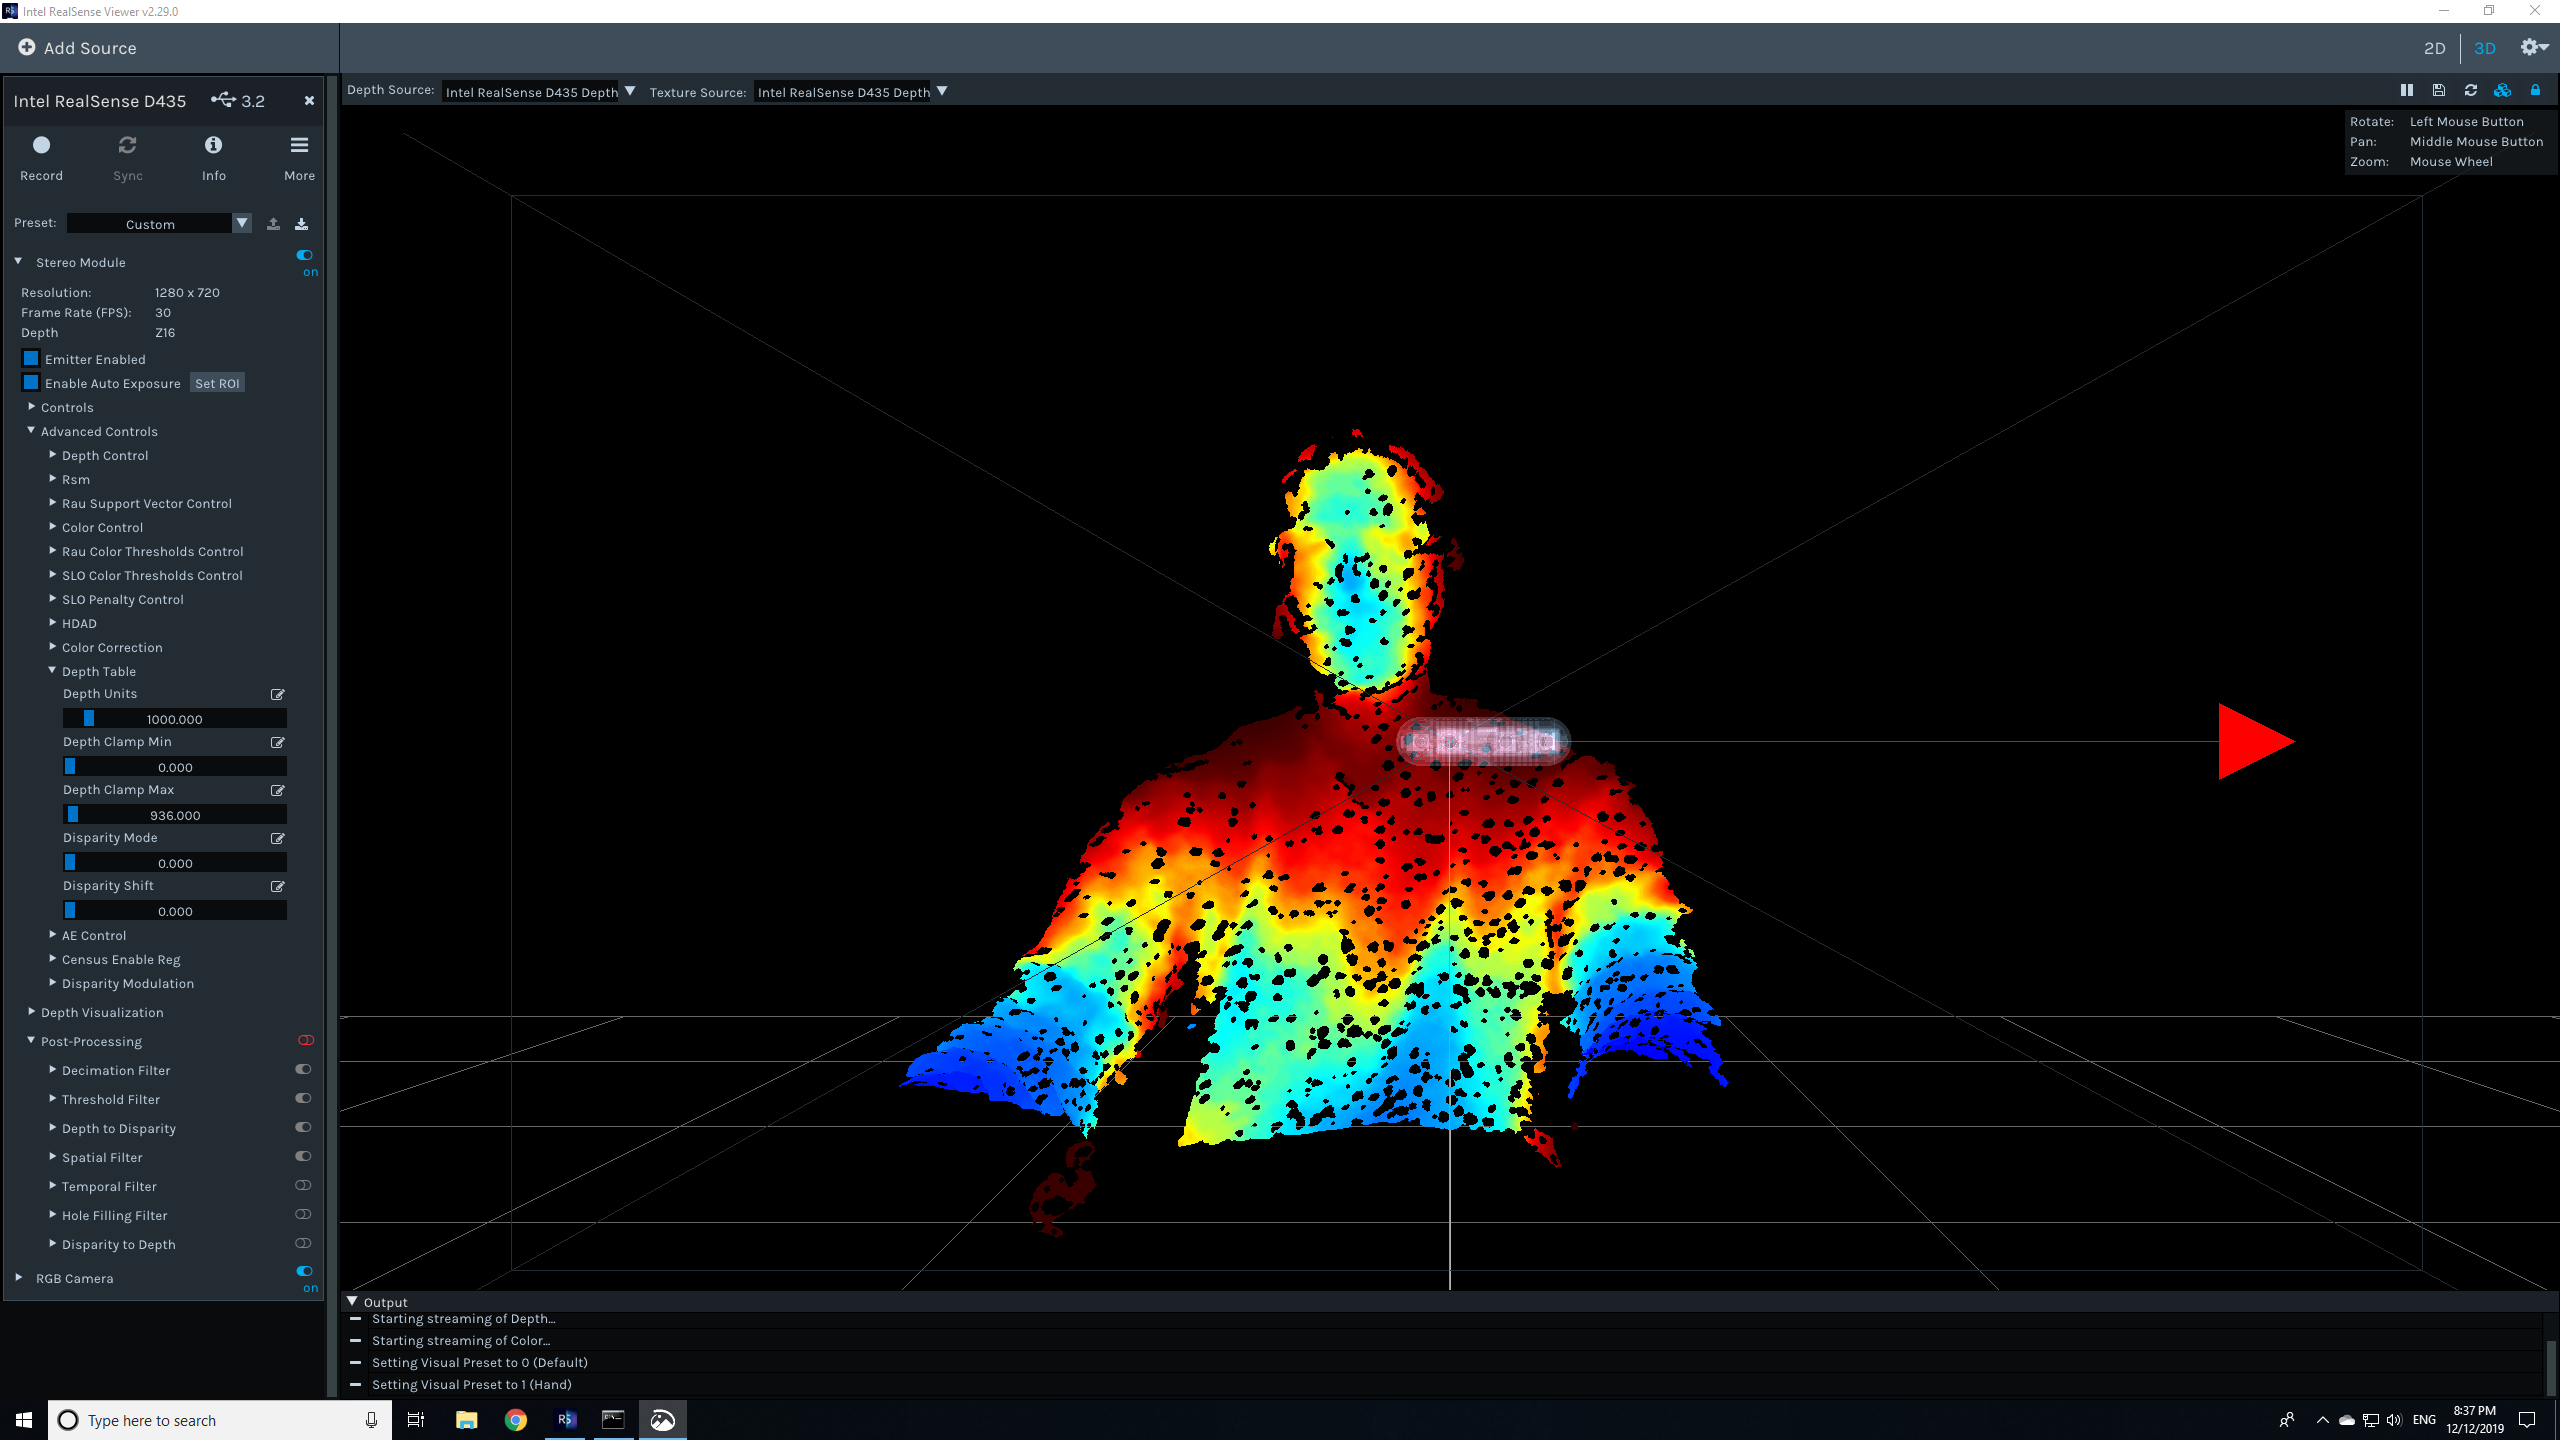
\includegraphics[width=0.3\textwidth]{without_post_processing.png}
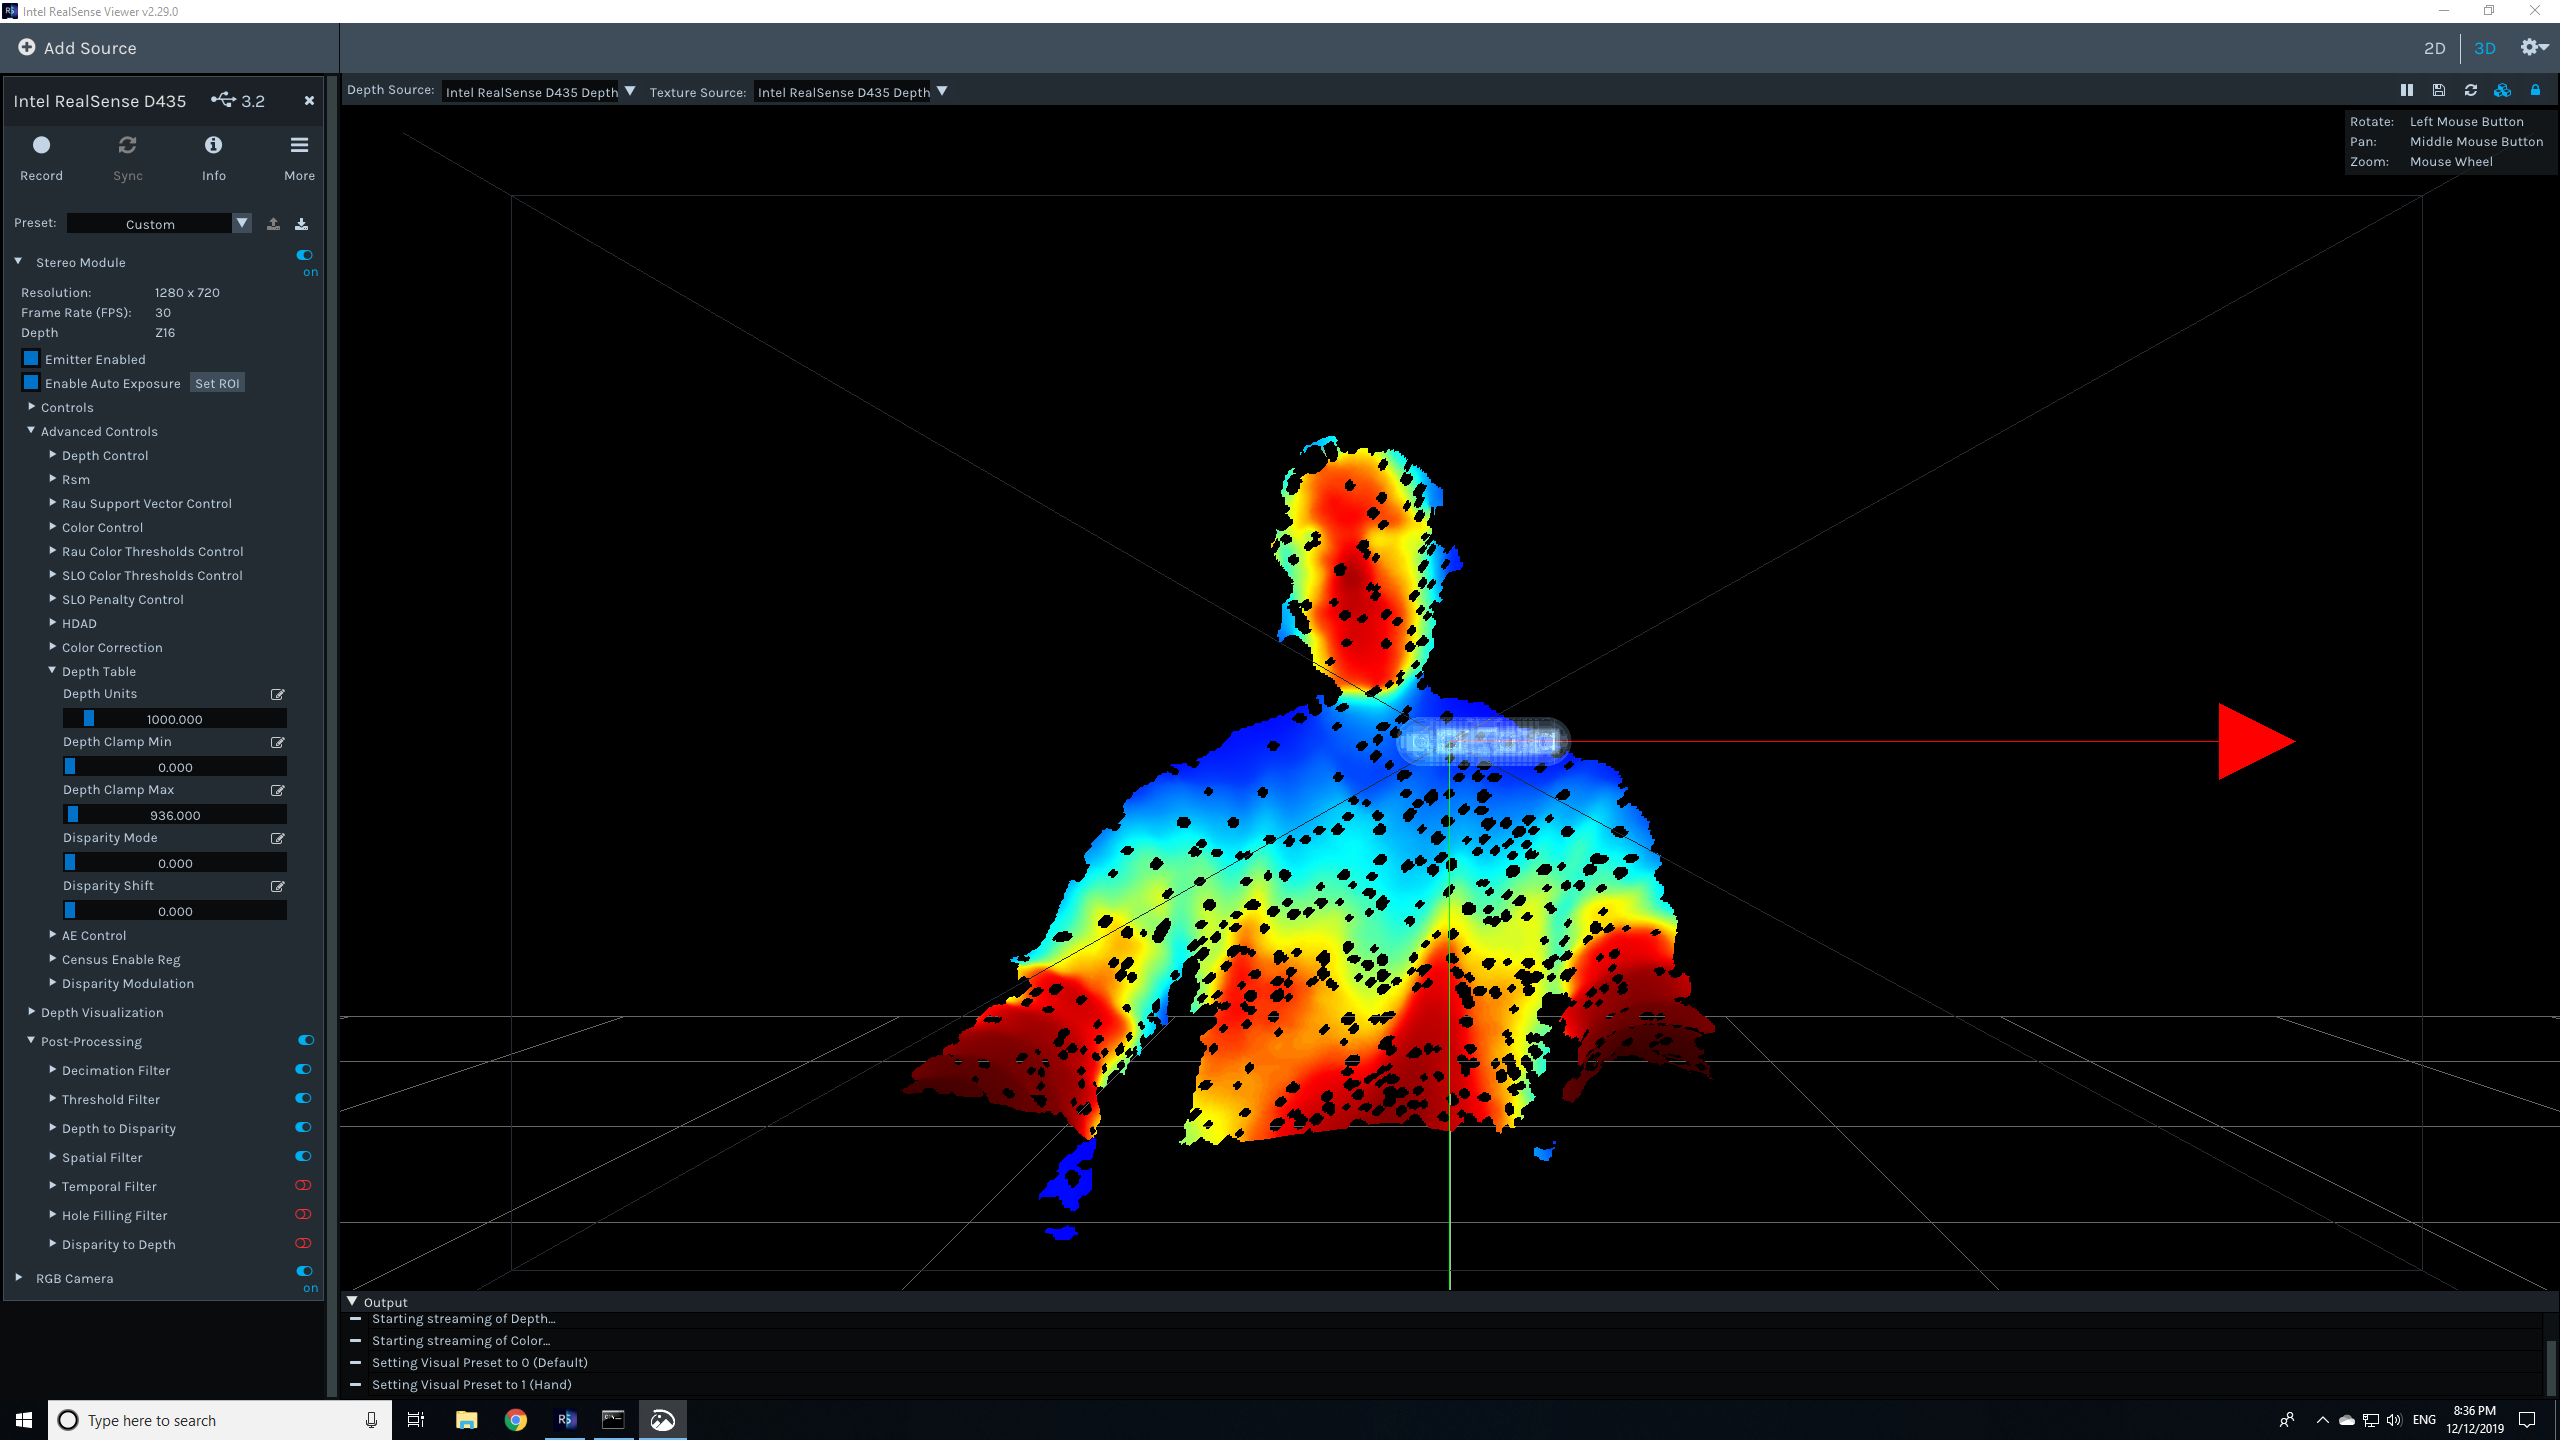
\includegraphics[width=0.3\textwidth]{with_spatial_filtering.png}
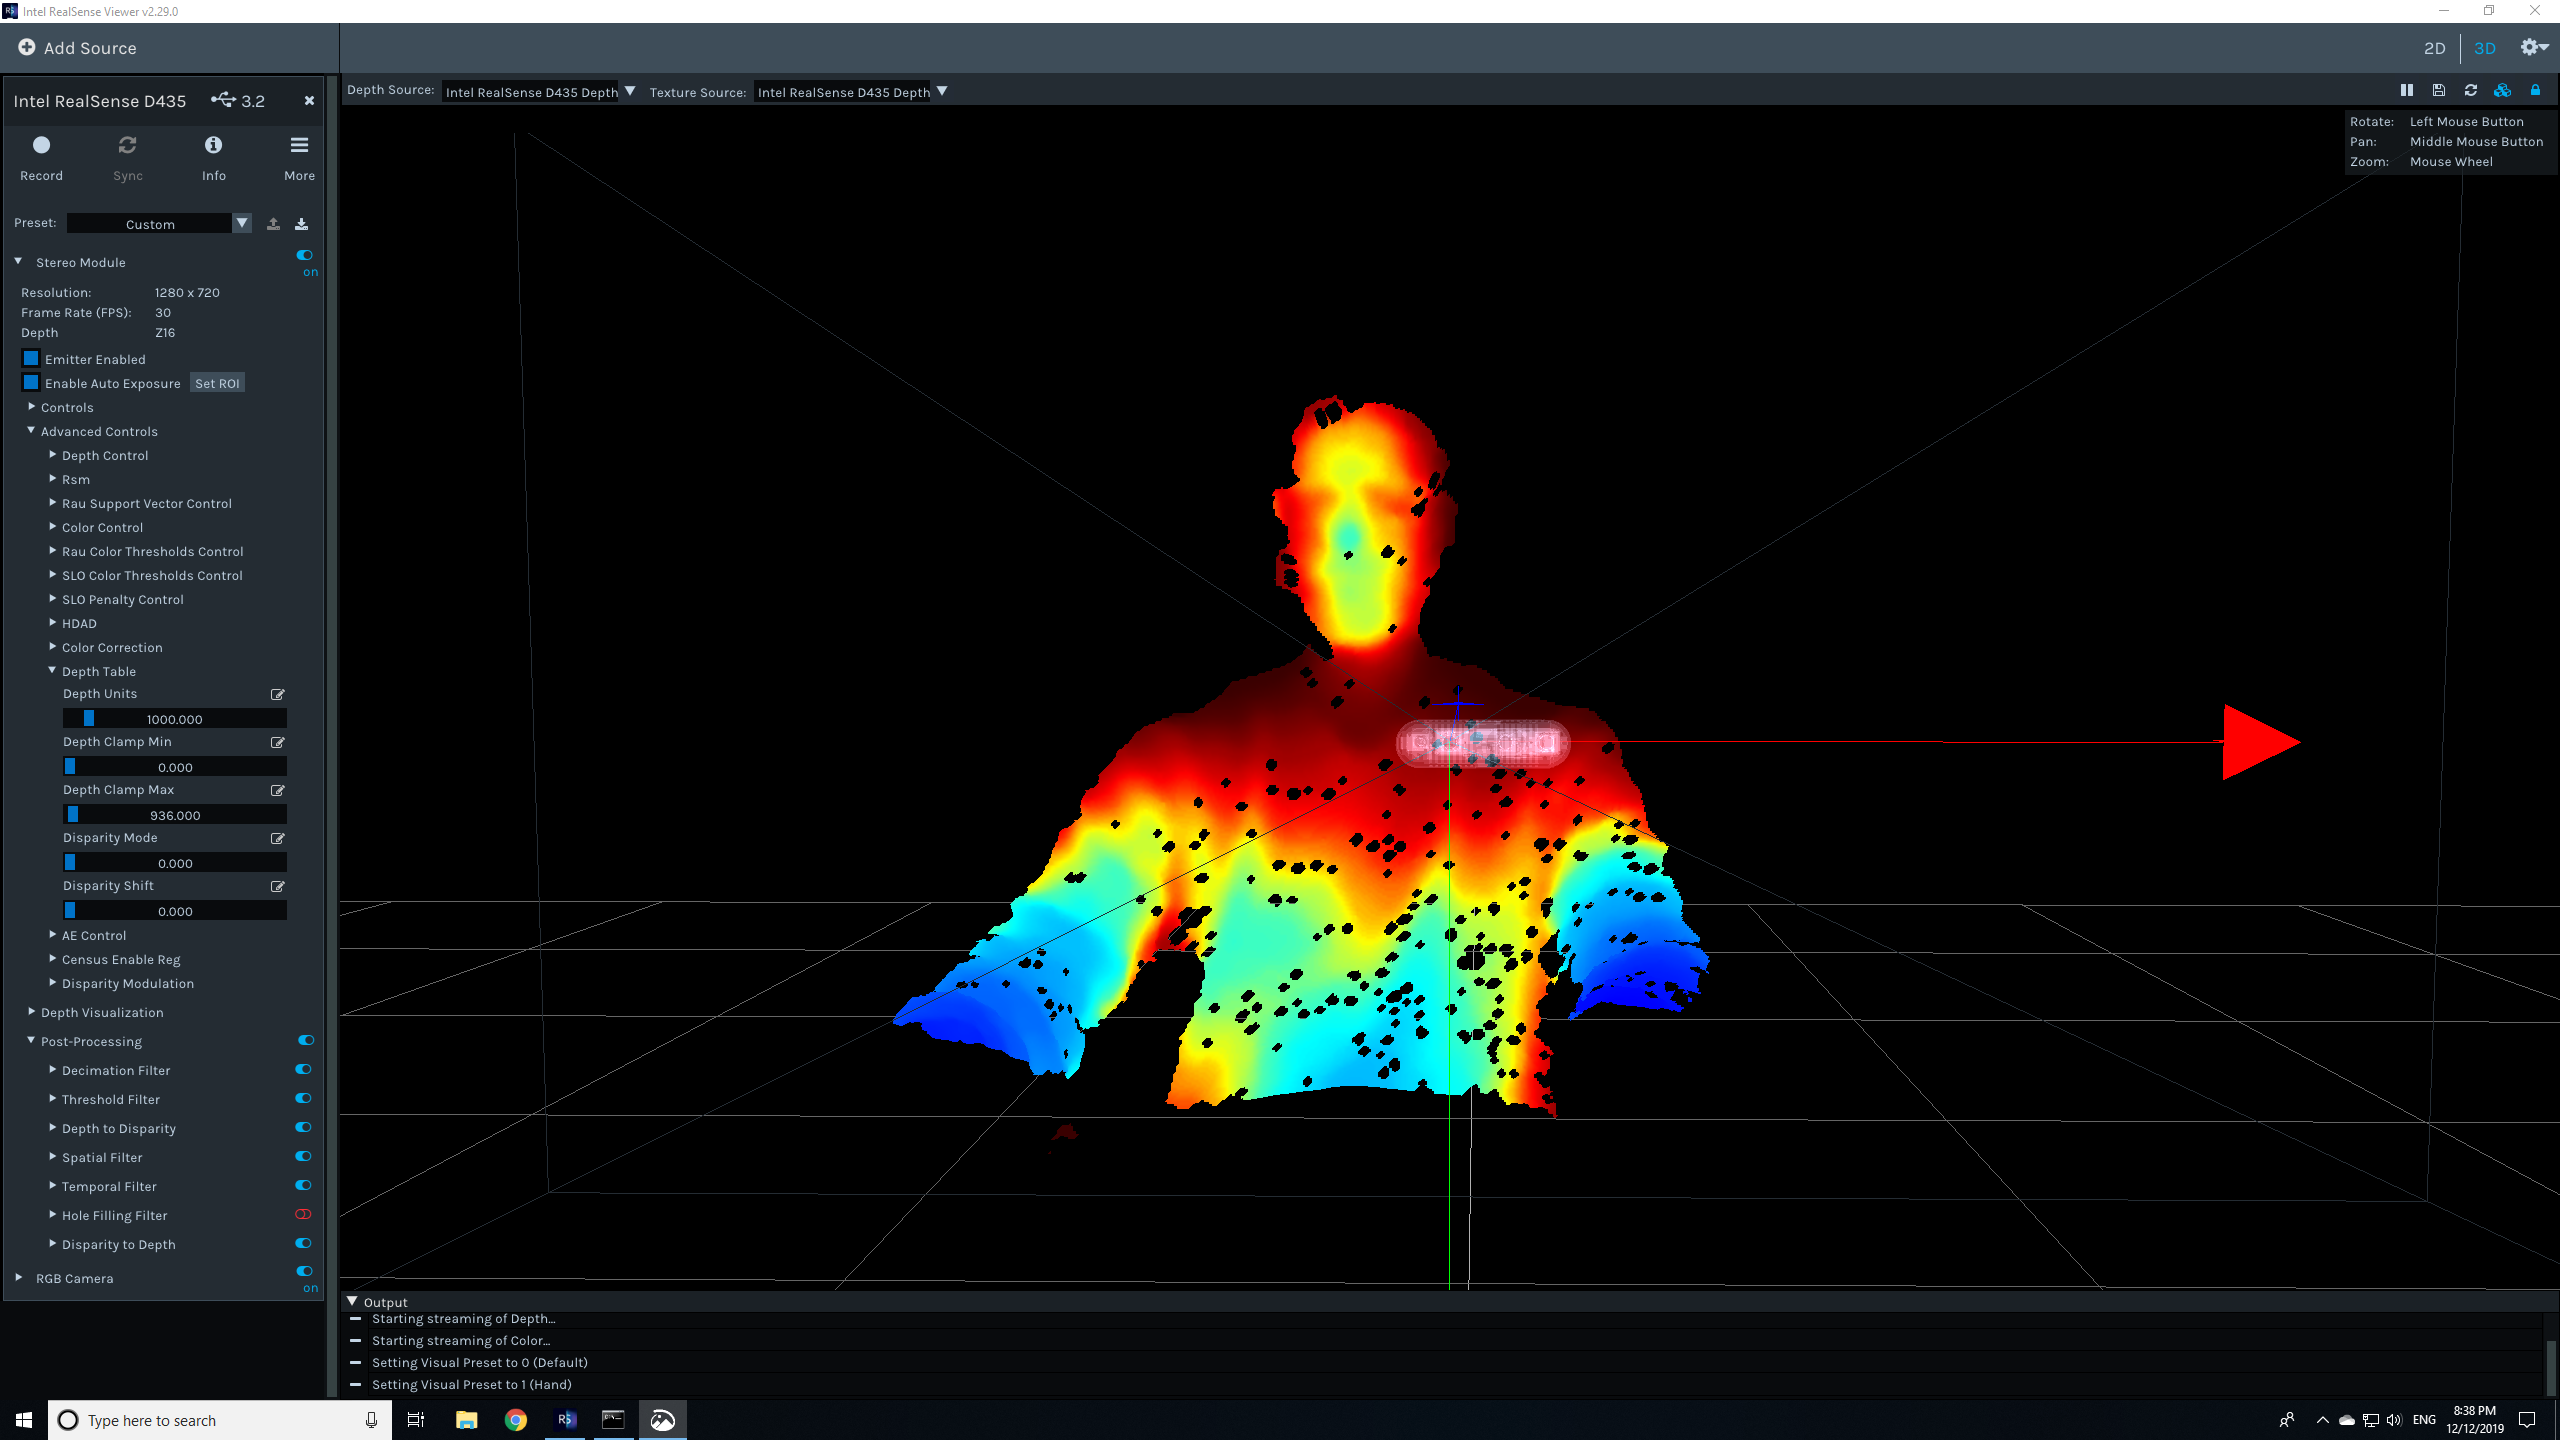
\includegraphics[width=0.3\textwidth]{with_all_processing_but_hole_filling.png}
\caption{Depth images captured without post processing (left), with spatial filtering (middle)
and using all available options (right)}
\end{figure}

Large-scale version of these images are included in an appendix.
\subsection{Removing Outliers and Errors}

Even with the background subtraction and filters, there are often still
outliers and errors that should not be included in a quality model. Worse still,
these garbage vertices make it harder to perform the registration in the next phase.
Luckily, MeshLab \cite{cignoni2008meshlab} makes it quite easy to select,
move and delete vertices.

\begin{figure}[h]
\centering
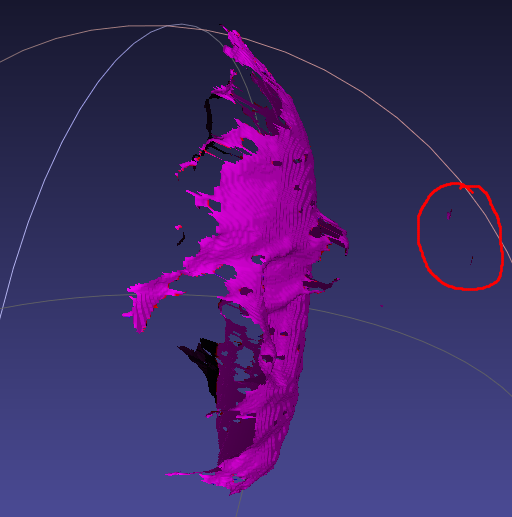
\includegraphics[width=0.45\textwidth]{outliers.png}
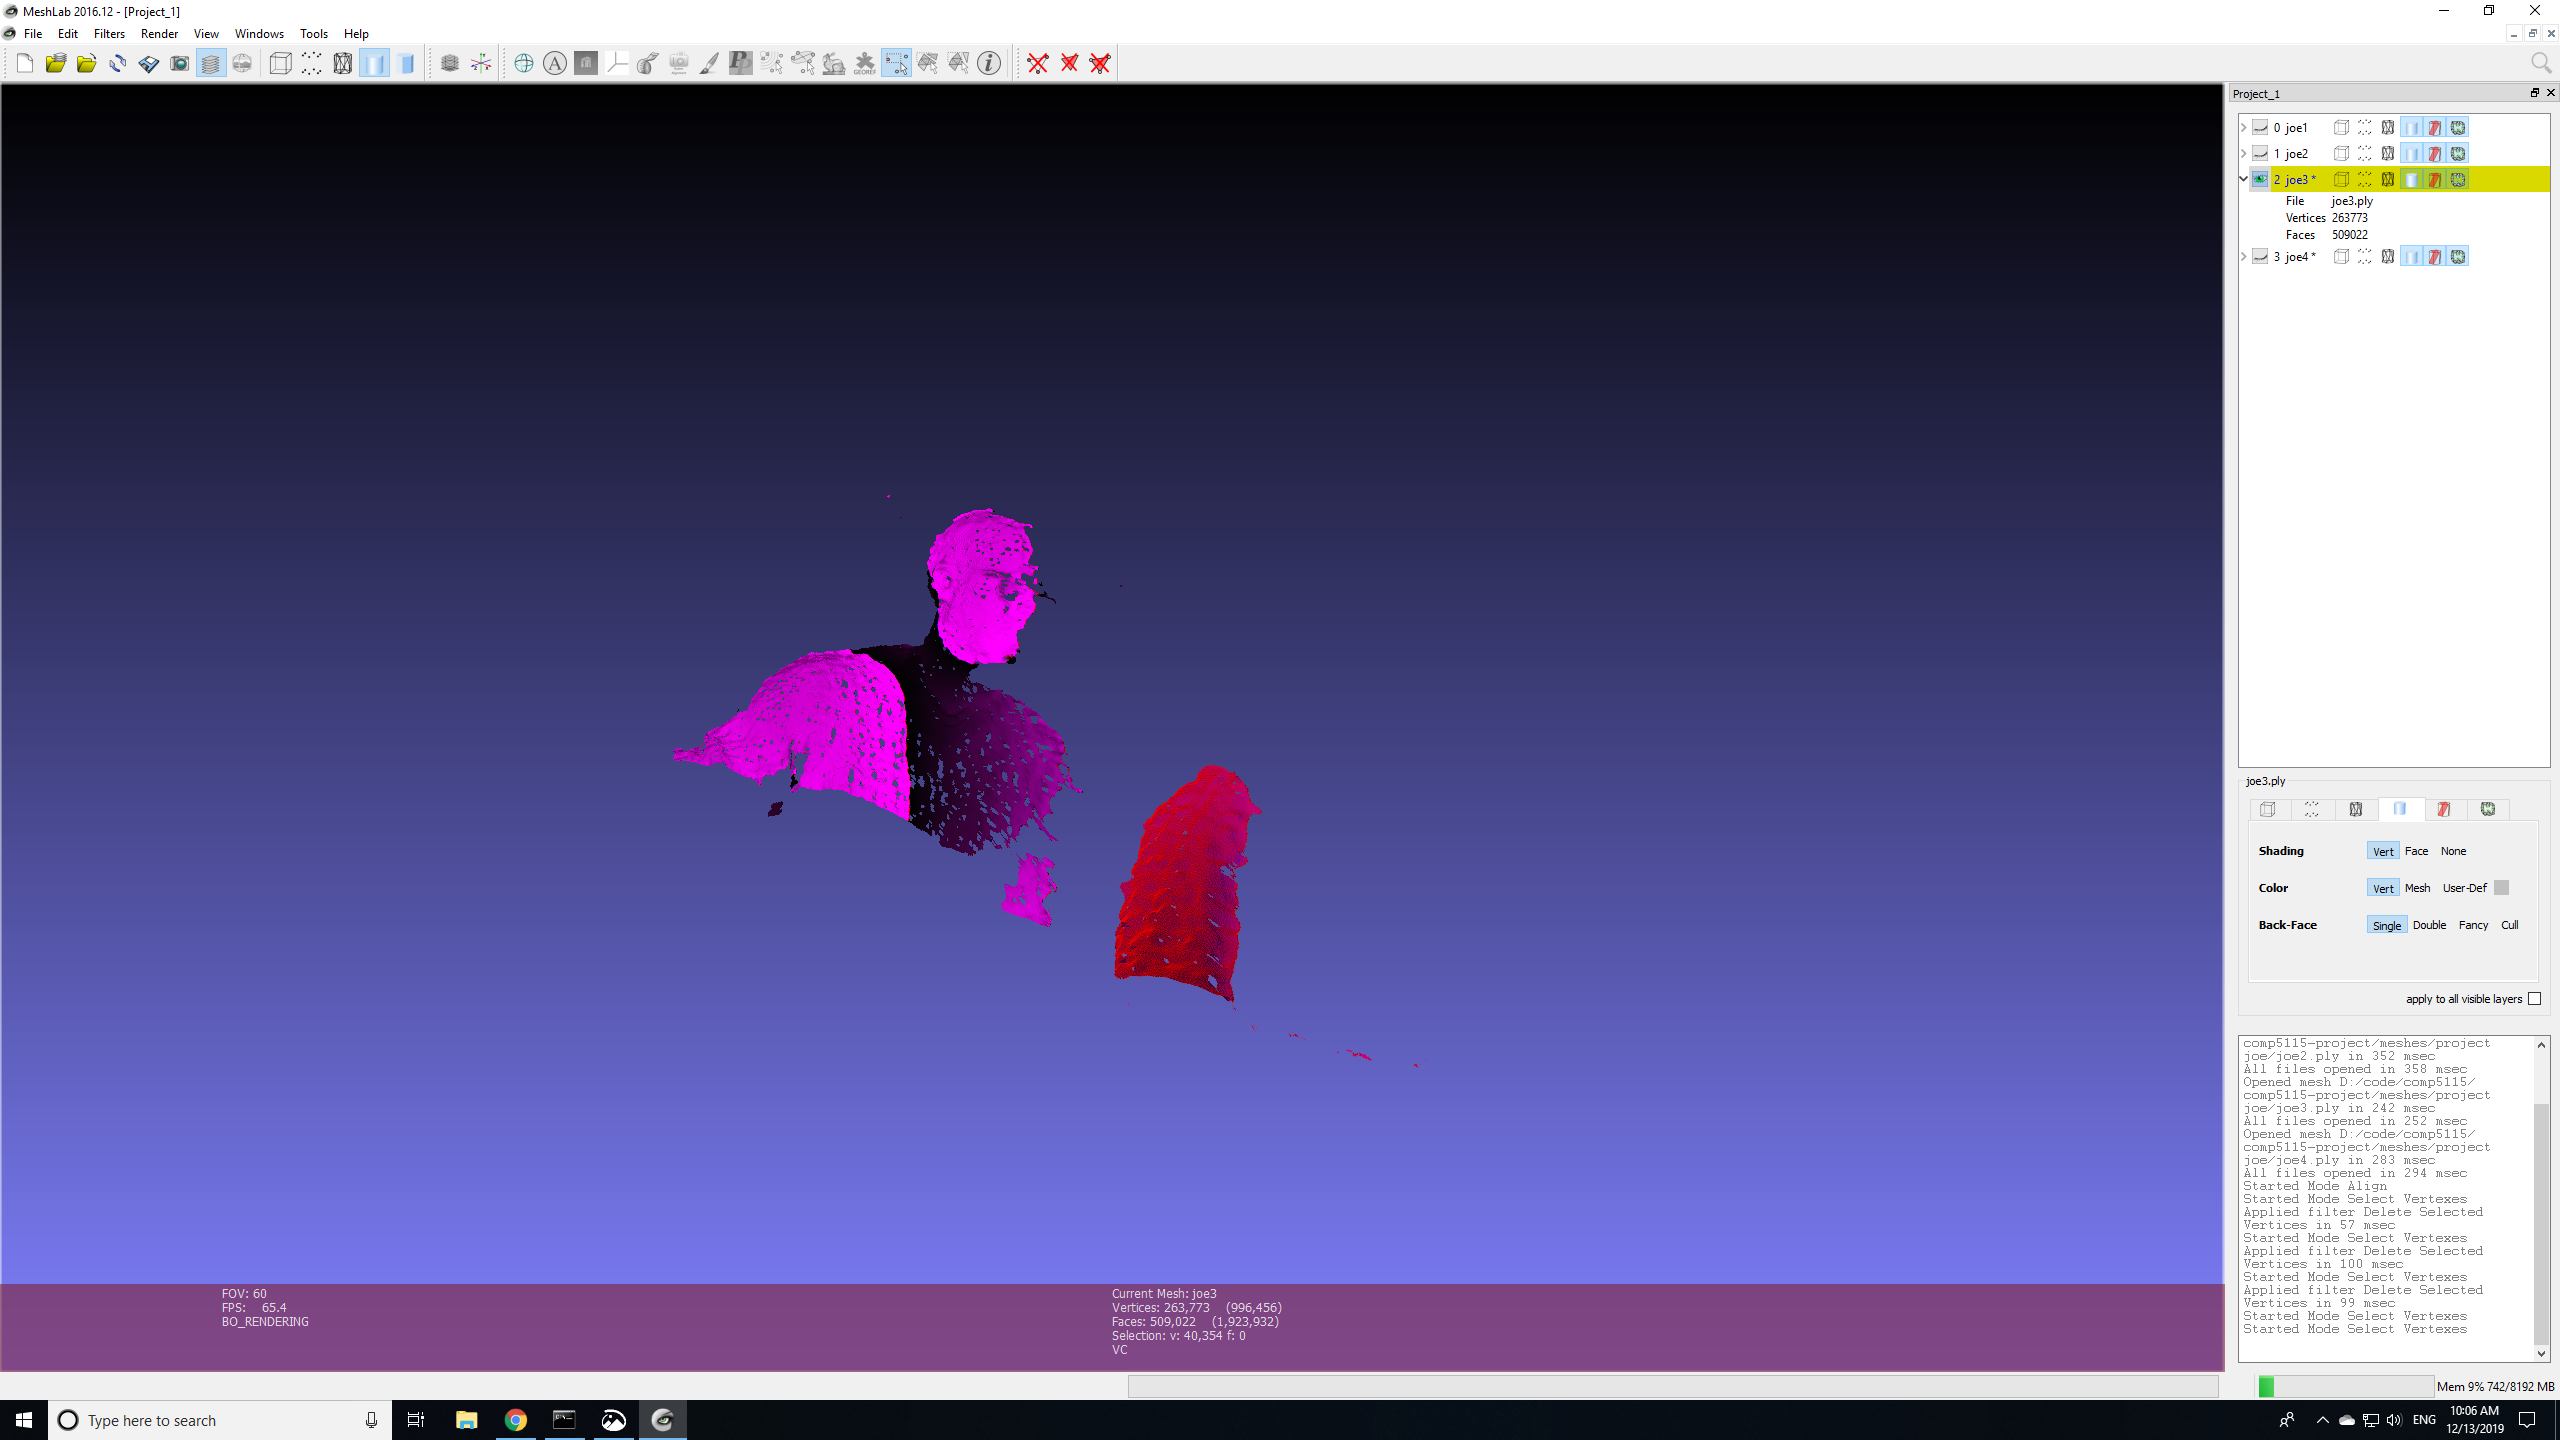
\includegraphics[width=0.45\textwidth]{removing_chair_from_layer.png}
\caption{Outliers caused by erroneous readings (left), removing chair from capture}
\end{figure}

One way to remove extraneous points is to use the connected component selection
tool to grab the object of interest, then use the selection inversion to select
every point except the model. All these vertices and/or faces can then be deleted.

This process needs to be repeated for each point cloud which will constitute
a ``layer'' in the model construction.

\subsection{Aligning Point Clouds}

Once cleaned, MeshLab \cite{cignoni2008meshlab} can be used to align the point clouds.
Each point cloud mesh is imported as its own layed, which can be moved and rotated so that
they lign up closely. This problem is also known as point cloud registration \cite{pomerleau2015review} and the Iterative
Closest Points (or ICP) is another well-studied algorithm. MeshLab provides a user-assisted
method for giving the ICP a head start by choosing an initial alignment.

In MeshLab, open the Alignment tool and Glue one of the layers as a base.
Now choose a different layer to align and select Point Based Gluing.
It opens a new window which allows the user to move and rotate the two clouds to better view
common areas. Then, the user selects (at least) four points corresponding points on
both of the models to find an initial alignment.
Often, this initial alignment is not correct and the user must try again
with different points.

\begin{figure}[h]
\centering
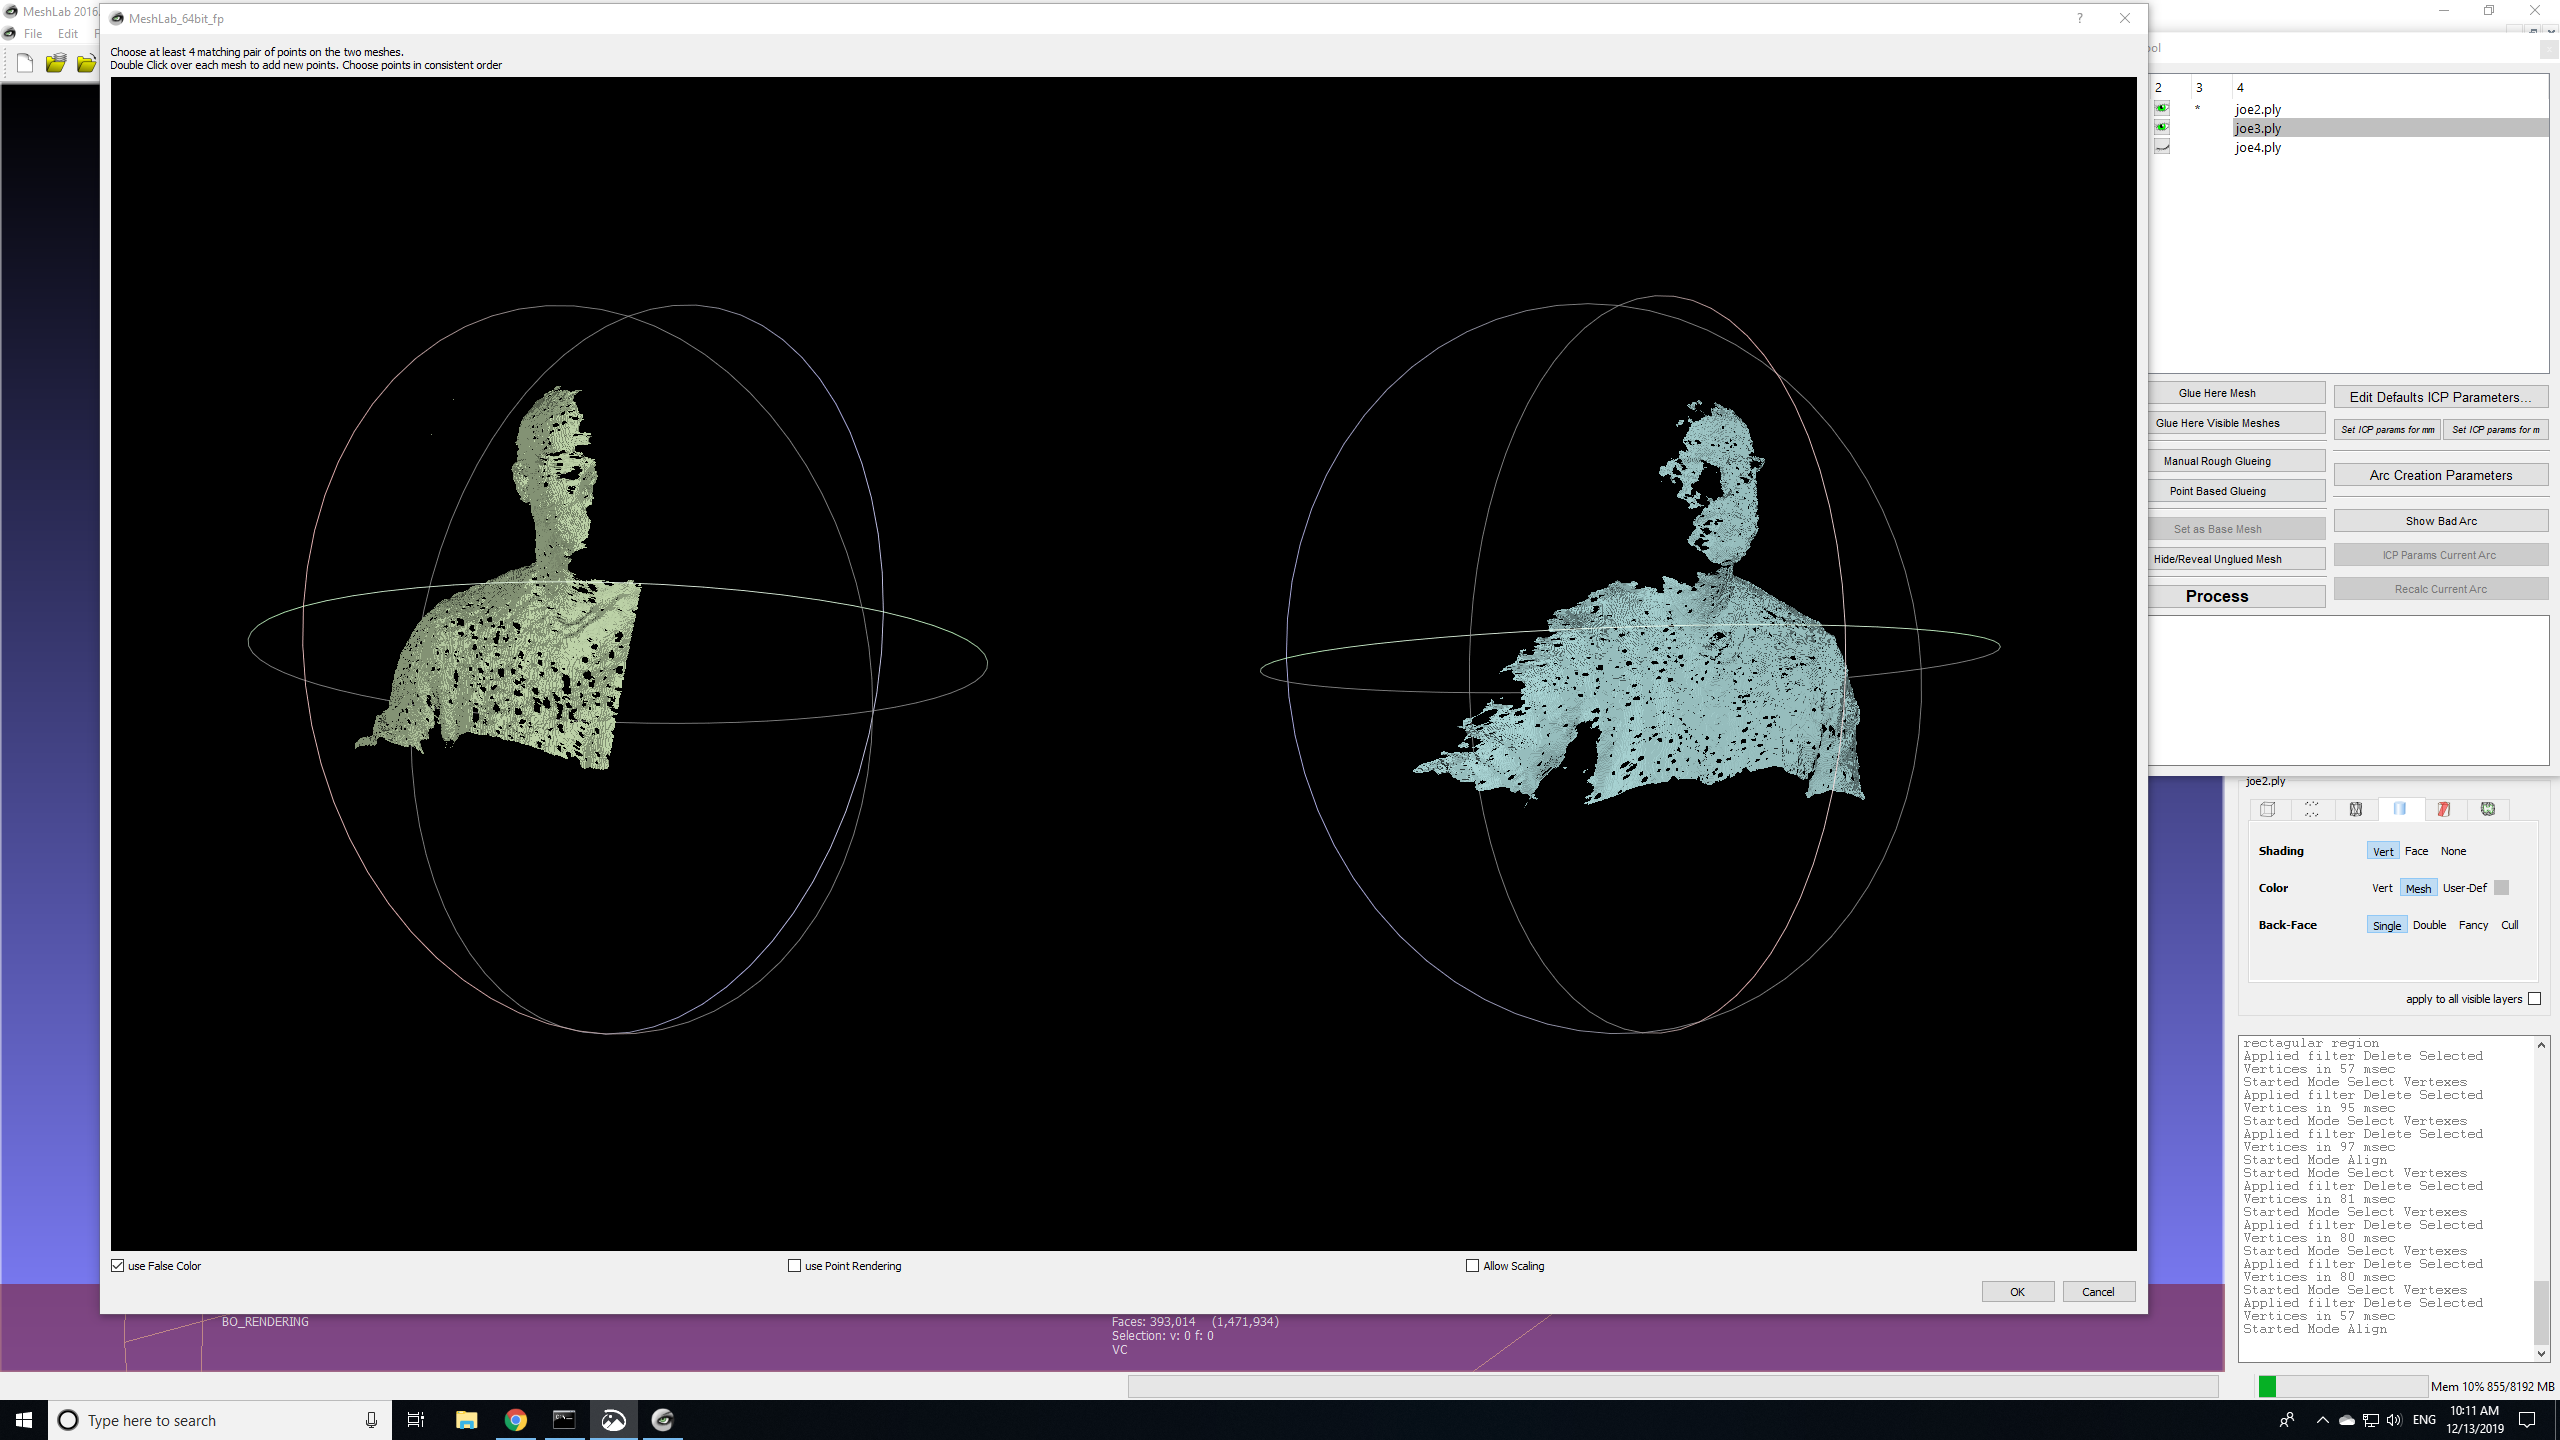
\includegraphics[width=0.6\textwidth]{align_two_clouds.png}
\caption{Point-based Initial Transform}
\end{figure}

Once an initial alignment is found, presssing Process in the Alignment window
runs Iterative Closest Points to refine the alignment. It is often helpful
to run the algorithm several times and/or increase the number of iterations in the
ICP parameters.

It can be particularly tricky to align two models with little in common. For a
quality point cloud, it would be necessary to take dozens if not hundreds
of captures so that the transition from each frame is smooth and common surface
between each one is maximized, especially if there are sharp edges as in the
Cube Man project.

\begin{figure}[h]
\centering
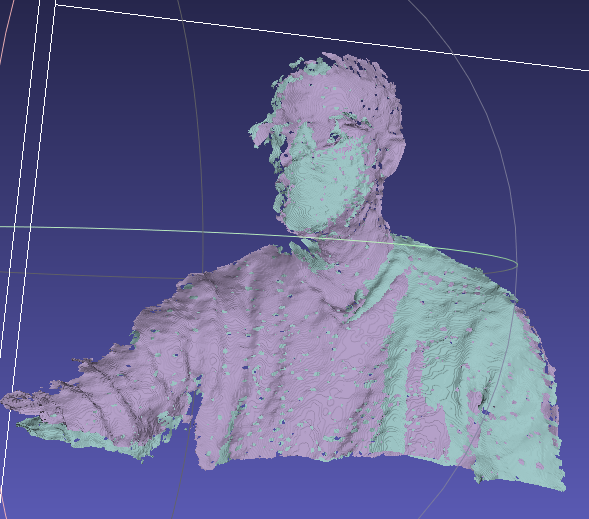
\includegraphics[width=0.6\textwidth]{two_clouds_merged.png}
\caption{Two point clouds aligned using ICP}
\end{figure}

After aligning two (or more) layers, you can then flatten them together by making
the aligned layers visible, right clicking in the layers window, and selecting
Flatten Visible Layers. Flattening the layers arguably makes it easier align additional
point clouds, since the known surface has hopefully expanded.

\subsection{Simplifications, Sampling and Smoothing}
Attempting reconstruction directly on the merged point clouds leads to fairly messy
objects. There are apparently non-manifold vertices and incorrect normals which produce strange
objects.

\begin{figure}[h]
\centering
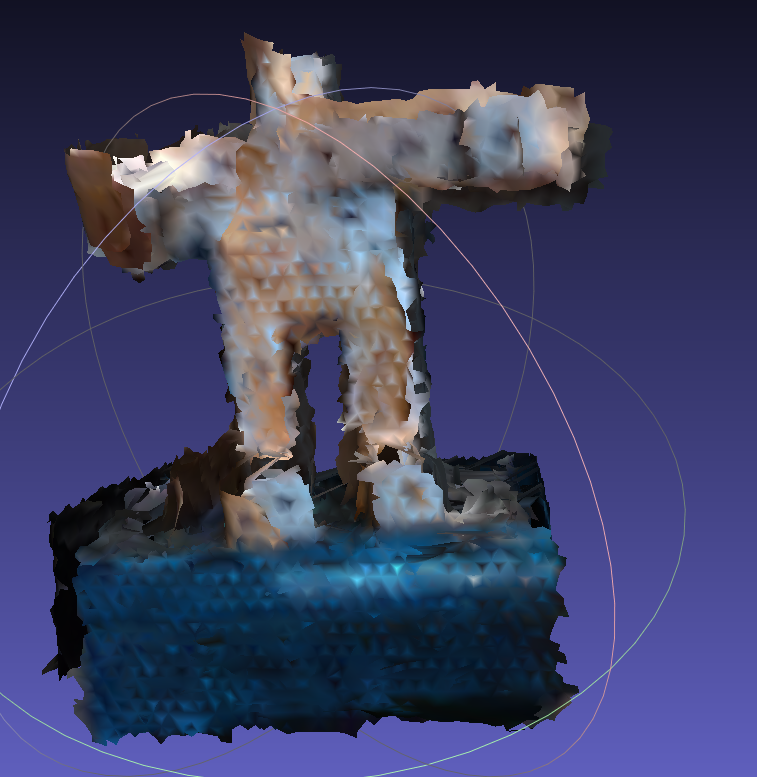
\includegraphics[width=0.6\textwidth]{clustering_decimation.png}
\caption{Simplifying merged cloud with clustering decimation}
\end{figure}
